\documentclass{amsart}

\usepackage[T1]{fontenc}
\usepackage{lmodern}
\usepackage{mathtools}
\usepackage{booktabs}
\usepackage{hyperref}
\usepackage{graphicx}
\usepackage{microtype}
\usepackage{tikz}
\usetikzlibrary{positioning,decorations.pathreplacing}

% ---------- theorem styles ----------
\newtheorem{theorem}{Theorem}[section]
\newtheorem{proposition}[theorem]{Proposition}
\newtheorem{corollary}[theorem]{Corollary}
\newtheorem{lemma}[theorem]{Lemma}
\newtheorem{conjecture}[theorem]{Conjecture}
\theoremstyle{definition}
\newtheorem{definition}[theorem]{Definition}
\theoremstyle{remark}
\newtheorem{remark}[theorem]{Remark}
\newtheorem{example}[theorem]{Example}

% ---------- notation ----------
\newcommand{\R}{\mathbb{R}}
\newcommand{\Z}{\mathbb{Z}}
\newcommand{\N}{\mathbb{N}}
\newcommand{\Q}{\mathbb{Q}}
\newcommand{\C}{\mathbb{C}}
\newcommand{\dH}{\dim_{\mathrm{H}}}
\title{Disk-Like Self-Similar Tiles with High Boundary Dimension}

\author{Dmitry Mekhontsev}
\address{Novosibirsk State University, Novosibirsk, Russia}
\email{mekhontsev@gmail.com}
\subjclass[2020]{28A80 (primary), 52C20, 37C70 (secondary)}
\keywords{Self-similar tile, boundary dimension, Hausdorff dimension,
  neighbor graph, disk-like tile}
\date{\today}

% --------------------------------------------------------------------------
\begin{document}

\begin{abstract}
We construct an infinite family of self-similar plane tiles
$\{A_n\}_{n \ge 3}$, each generated by $n$~contractions of
ratio~$1/\!\sqrt{n}$, with the following properties:
(i)~the neighbor graph has exactly $6$~boundary components for
every~$n$;
(ii)~each $A_n$ is disk-like (homeomorphic to a closed disk);
(iii)~the boundary Hausdorff dimension satisfies
$\dH(\partial A_n) = 2\log\lambda_n/\log n$, where $\lambda_n$ is
the dominant root of an explicit quartic polynomial
$p_n(x) = x^4 - (n{-}1)x^3 - 2x^2 - (n{-}1)(n{-}4)x + n(n{-}2)$,
and $2 - \dH(\partial A_n) \sim 8/(n^2\ln n)$ as $n \to \infty$.
In particular, $\dH(\partial A_n) \to 2$ with bounded neighbor
graph complexity.  Despite the increasingly rough boundary,
the tiling has the combinatorial type of a regular hexagonal
tiling for every~$n$: each tile has $6$ edge neighbors and
$6$ triple points, all of valence~$3$.
This complements the examples of
Keesling~\cite{keesling}, where $\dH(\partial A) \to n$
in~$\R^n$ but the graph complexity grows without bound.
The construction generalises to~$\R^d$: the closed-form case
$d = 1$ and exact computations for $d \le 7$ suggest that the
number of boundary components is $\tfrac{1}{2}\bigl((1{+}\sqrt 2)^{d+1}
+ (1{-}\sqrt 2)^{d+1}\bigr) - 1$, and
$d - \dH(\partial A_n) \sim 2d^2/(n^2\ln n)$.
\end{abstract}

\maketitle

% --------------------------------------------------------------------------
\section{Introduction}
\label{sec:intro}

A \emph{self-similar tile} is a compact set $A \subset \R^2$ with
non-empty interior satisfying
\[
  A = \bigcup_{i=0}^{N-1} f_i(A),
\]
where the $f_i$ are contractive similarities~\cite{hutchinson} and the union is
measure-disjoint (the \emph{Open Set Condition}, hereafter OSC).
Such tiles arise naturally in the study of
self-affine lattice tilings~\cite{lagarias-wang}.
The \emph{boundary} $\partial A$ is a compact fractal set whose
Hausdorff dimension $s = \dH(\partial A)$ satisfies
$1 \le s < 2$
(see~\cite{falconer} for background on Hausdorff dimension).

\textbf{Achieving $\dH(\partial A)$ close to $2$ is easy in principle.}
Keesling~\cite{keesling} proved that $\dH(\partial A) < n$ for every
self-similar tile in~$\R^n$ and gave examples showing that $\dH(\partial A)$
can be arbitrarily close to~$n$
(see also Duvall, Keesling and Strichartz~\cite{duvall-keesling-strichartz}
for explicit calculations of boundary dimensions).  In those examples the IFS has $4k{+}3$
maps on~$\R$ with every fourth digit offset, and the number of boundary
components (the \emph{neighbor graph complexity}) grows without bound
as $k \to \infty$.

\textbf{The disk-like constraint is much more restrictive.}
High boundary dimension corresponds to extreme geometric roughness of
$\partial A$, and tiles with large $\dH(\partial A)$ are generically
non-disk-like (e.g., the L{\'e}vy~C curve with
$\dH(\partial A) \approx 1.934$ is not a topological disk).
Achieving $\dH(\partial A)$ close to~$2$ while maintaining the
disk-like property and bounded graph complexity is therefore a much
harder problem.

The natural question arises: \emph{can $\dH(\partial A)$ approach~$2$
with a bounded number of boundary components and the disk-like property?}

\textbf{Main result (informal).}
For every integer $n \ge 3$ there is a self-similar plane tile $A_n$,
defined by $n$~contractions of ratio $1/\!\sqrt{n}$
(Definition~\ref{def:comb}), such that:
\begin{itemize}
\item[(a)] \emph{Bounded graph complexity:} the neighbor graph of $A_n$
  has exactly $6$~boundary components, independent of~$n$
  (Theorem~\ref{thm:graph}).
\item[(b)] \emph{Disk-likeness:} $A_n$ is homeomorphic to the closed
  disk, and the tiling has the combinatorial type of the regular
  hexagonal tiling: each tile has $6$~edge neighbors and $6$~triple
  points of valence~$3$ (Theorem~\ref{thm:disklike},
  Remark~\ref{rem:topology}).
\item[(c)] \emph{Boundary dimension tends to~$2$:} the boundary
  dimension is given by $\dH(\partial A_n) = 2\log\lambda_n / \log n$
  where $\lambda_n$ is the dominant real root of the explicit quartic
  \[
    p_n(x) = x^4 - (n{-}1)x^3 - 2x^2 - (n{-}1)(n{-}4)x + n(n{-}2);
  \]
  consequently $2 - \dH(\partial A_n) \sim 8/(n^2\ln n)$
  as $n\to\infty$ (Theorems~\ref{thm:dim} and~\ref{thm:asymp}).
\end{itemize}
All three properties are proved by an explicit analysis of the
refinement equation; the proofs are uniform in~$n$.  A generalisation
to~$\R^d$ is developed in Section~\ref{sec:higherdim}, together with
the closed-form case $d = 1$ (\S\ref{ssec:d1}) and conjectures
supported by exact computation for $d \le 7$.

\textbf{Discovery.}
The family was found by a systematic computational search over IFS with
companion matrices and mixed orientation assignments, using
IFStile~\cite{ifstile} to evaluate the neighbor graph and boundary
dimension for each candidate.  The key structural observation --- that
$n{-}1$ collinear contraction maps of equal ratio plus one transverse
map with opposite orientation yield a constant $6$-component neighbor
graph for every~$n$ --- emerged from this search and was subsequently
verified by the purely analytic proofs of
Sections~\ref{sec:osc}--\ref{sec:disklike}.

\subsection*{Related work}

The comb family sits at the intersection of three strands of the
literature.

\emph{Topology and disk-likeness of self-similar tiles.}
General criteria for a planar self-affine tile to be homeomorphic to
a disk were developed by Bandt and Wang~\cite{bandt-wang}, with
further refinements by Leung and Lau~\cite{leung-lau} and Ngai and
Tang~\cite{ngai-tang}; we rely on the neighbor-based criterion of
Loridant, Luo and Thuswaldner~\cite{loridant-luo-thuswaldner}.
A broader survey of topological properties of tiles arising from
number systems is given by Akiyama and
Thuswaldner~\cite{akiyama-thuswaldner}.

\emph{Boundary dimension.}
The computation of $\dH(\partial A)$ for a self-similar tile reduces
to the spectral radius of a graph-directed substitution
matrix~\cite{mauldin-williams}, whose construction via the neighbor
graph was systematised by Scheicher and
Thuswaldner~\cite{scheicher-thuswaldner}; explicit calculations for
specific families appear in Duvall, Keesling and
Strichartz~\cite{duvall-keesling-strichartz}.  Keesling's
bound~\cite{keesling} $\dH(\partial A) < n$ for tiles in~$\R^n$
together with his examples approaching this bound provide the
upper-dimension envelope within which our construction lives.

\emph{Self-affine tilings and separation.}
The broader setting of self-affine lattice tilings is due to
Bandt~\cite{bandt1991} and Lagarias and Wang~\cite{lagarias-wang};
the Open Set Condition and its weakenings are studied by Lau and
Ngai~\cite{lau-ngai}.  Our IFS is self-similar in the strict sense
(equal contraction ratios, orthogonal matrices), so OSC and the
classical Moran formula apply directly.

\subsection*{Why this family was not found earlier}

Existing constructions of self-similar planar tiles fall into two
broad classes.  \emph{Number-system tiles}~\cite{akiyama-thuswaldner,
lagarias-wang} use a fixed expansion matrix together with a digit
set forming a complete residue system in a quadratic ring such as
$\Z[i]$ or $\Z[\omega]$; all digit maps share the linear part~$+I$.
\emph{Symmetric IFS}~\cite{bandt-wang,duvall-keesling-strichartz}
arrange the digits cyclically (twindragon, terdragon, McMullen
carpets, etc.), so the boundary substitution matrix inherits a
discrete rotational or reflective symmetry that bounds its
spectral radius and confines $\dH(\partial A)$ well below the
ambient dimension.

The comb family departs from both schemes.  Its $n{-}1$ collinear
``spine'' digits use $+I$, while a single ``tooth'' digit uses
$-I$ with a transverse offset $2n{-}3$ tuned per~$n$.  This
asymmetric digit set, the use of two different linear parts, and
the dependence of the off-axis offset on the parameter~$n$ all
fall outside the symmetry assumptions that have implicitly
guided previous searches; in particular, no principled
derivation of the offset $2n{-}3$ is currently known
(see~\S\ref{sec:discussion}).  The construction was discovered by
an automated search over self-similar IFS minimising the
neighbour graph using the IFStile package~\cite{ifstile} and is
verified analytically here.

% --------------------------------------------------------------------------
\section{The Comb Family}
\label{sec:comb}

\subsection{Definition via companion matrix}

For an integer $n \ge 3$, consider the companion matrix
of the polynomial $x^2 - n$:
\begin{equation}\label{eq:companion}
  g = \begin{pmatrix} 0 & n \\ 1 & 0 \end{pmatrix},
\end{equation}
with eigenvalues $\pm\sqrt{n}$ and spectral radius $\sqrt{n}$.

\begin{definition}[Comb IFS]\label{def:comb}
For $n \ge 3$, the \emph{comb IFS with parameter~$n$} consists of $n$
digit maps acting on $\R^2$:
\begin{equation}\label{eq:comb-maps}
\begin{aligned}
  h_j(x) &= x + \bigl(j(n{-}1),\, 0\bigr), &\quad j = 0, 1, \ldots, n{-}2, \\
  h_{n-1}(x) &= -x + \bigl(n^2{-}n{-}1,\; 2n{-}3\bigr),
\end{aligned}
\end{equation}
with attractor
\begin{equation}\label{eq:attractor}
  A_n = g^{-1}\bigl(h_0(A_n) \cup h_1(A_n) \cup \cdots \cup h_{n-1}(A_n)\bigr).
\end{equation}
All digits are integer vectors.  The map $h_{n-1}$ includes a central
reflection $x \mapsto -x$.
\end{definition}

\begin{figure}[ht]
\centering
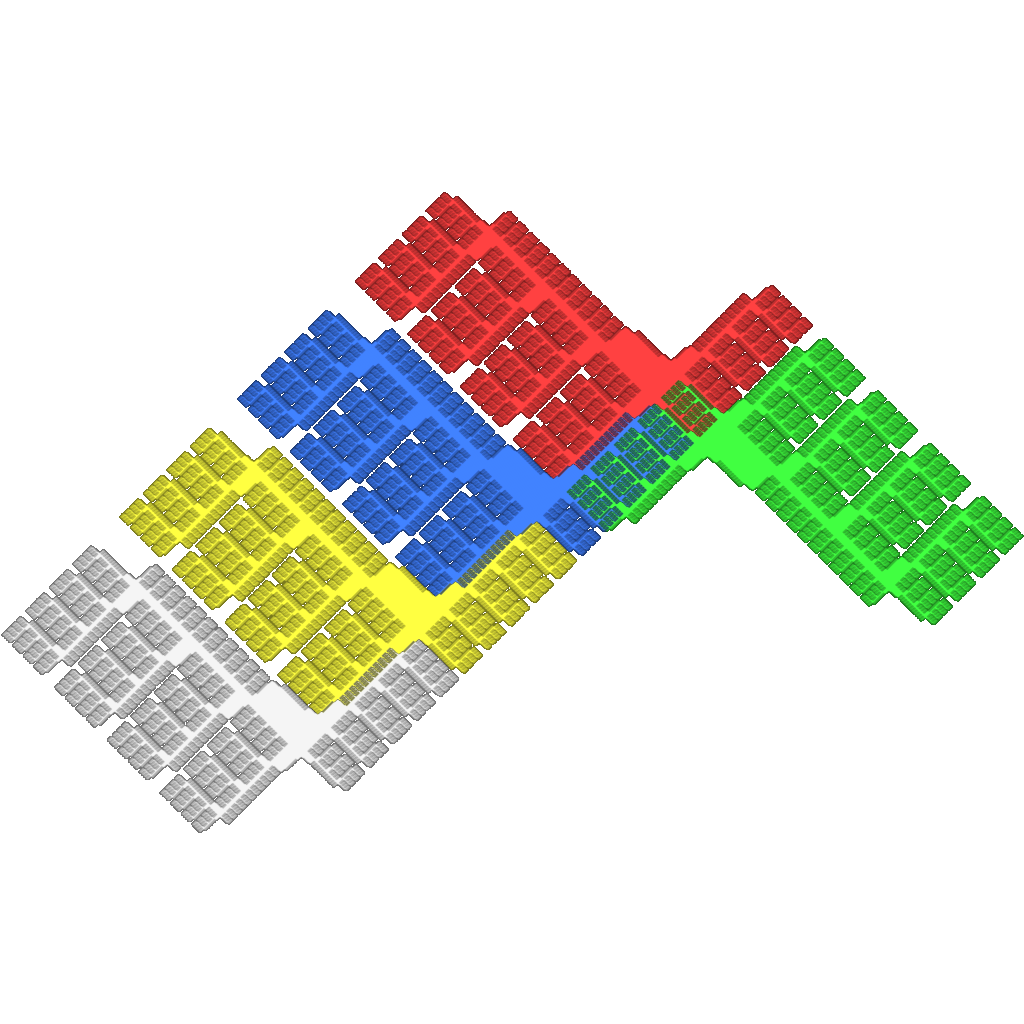
\includegraphics[width=0.65\textwidth]{comb-tile-n5.png}
\caption{The comb tile $A_5$ ($n = 5$, five maps).  Each first-level
  piece $f_j(A_5)$ is shown in a distinct colour: the four spine pieces
  $f_0, \ldots, f_3$ tile the lower-left staircase, while the single
  tooth piece $f_4$ (with central reflection) extends to the upper right.}
\label{fig:comb-tile}
\end{figure}

\begin{figure}[ht]
\centering
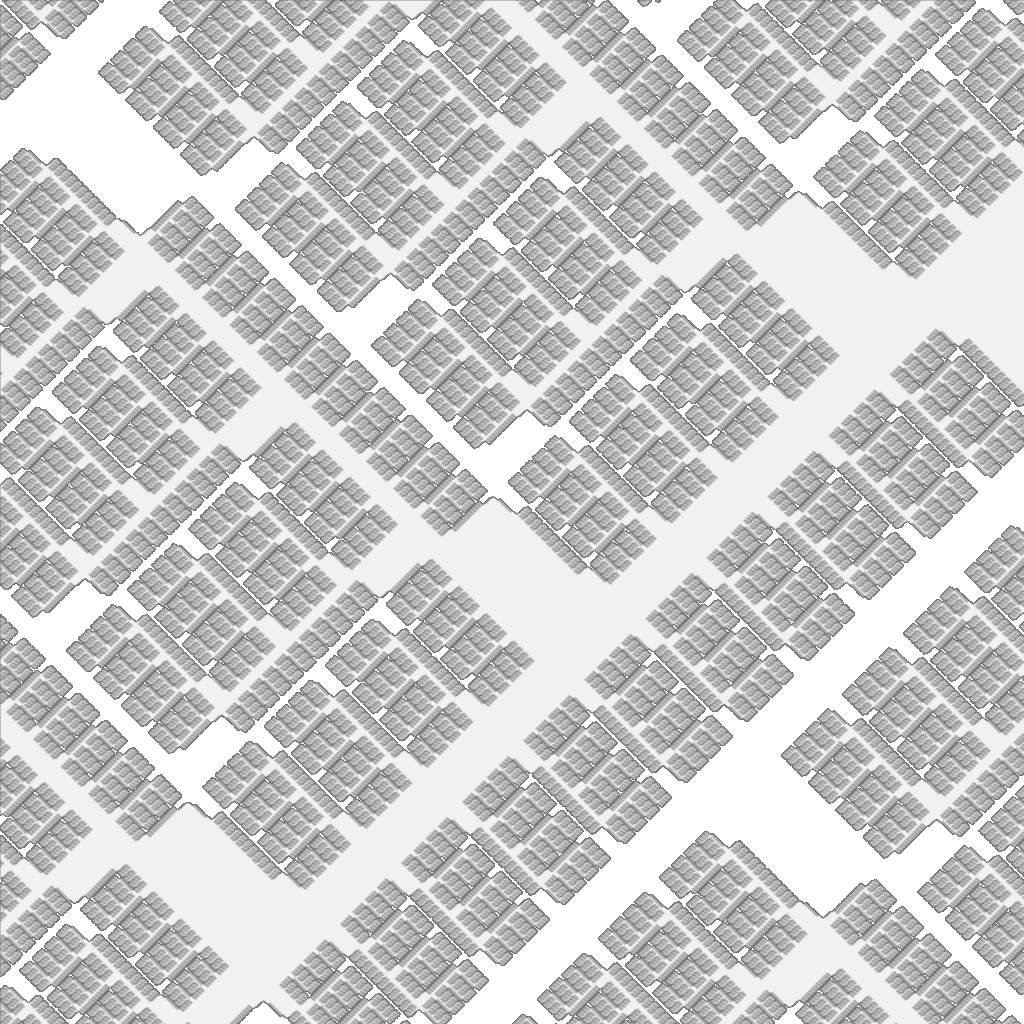
\includegraphics[width=0.55\textwidth]{comb-tile-n5-zoom.png}
\caption{Magnified fragment of the boundary $\partial A_5$.
  The boundary is a Jordan curve ($A_5$ is disk-like by
  Theorem~\ref{thm:disklike}), yet its Hausdorff dimension is
  $\dH(\partial A_5) \approx 1.863$ --- visibly close to
  space-filling.}
\label{fig:comb-zoom}
\end{figure}

\begin{figure}[ht]
\centering
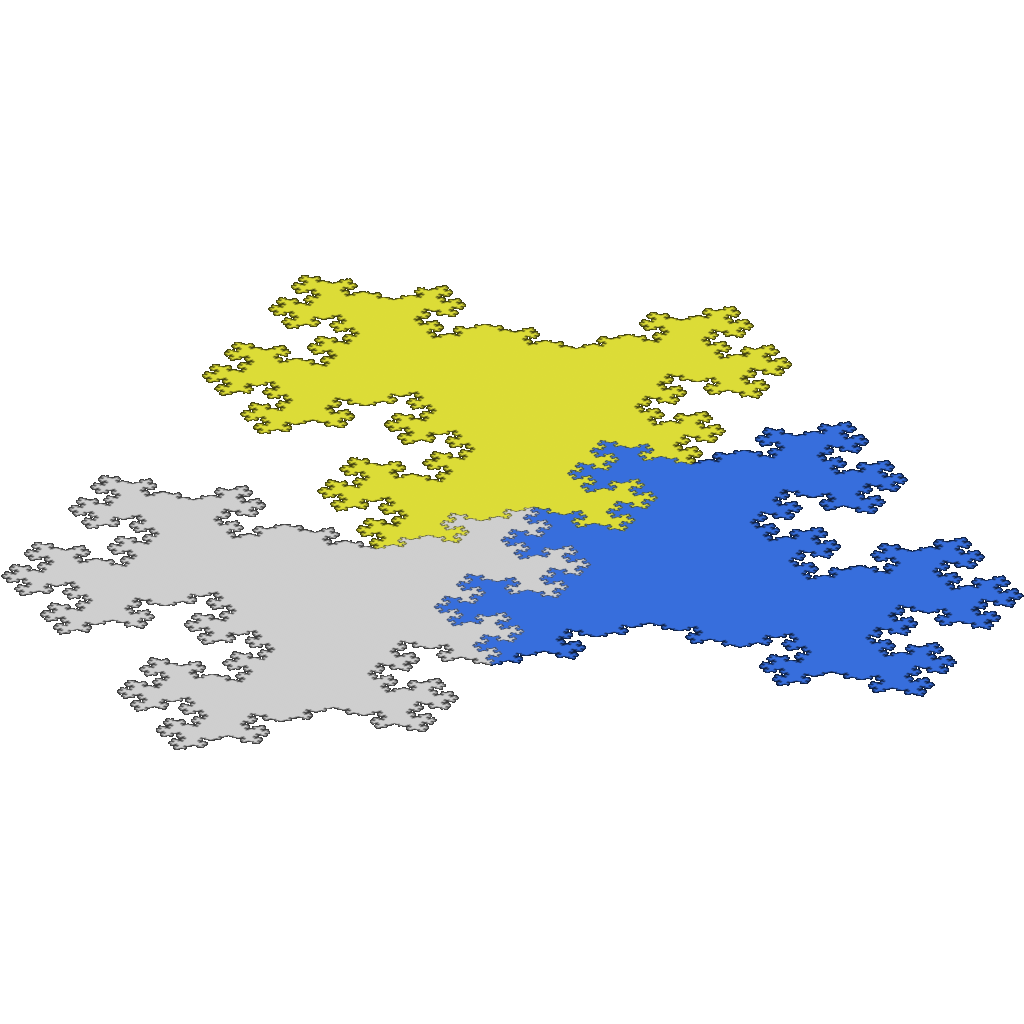
\includegraphics[width=0.48\textwidth]{comb-tile-n3.png}\hfill
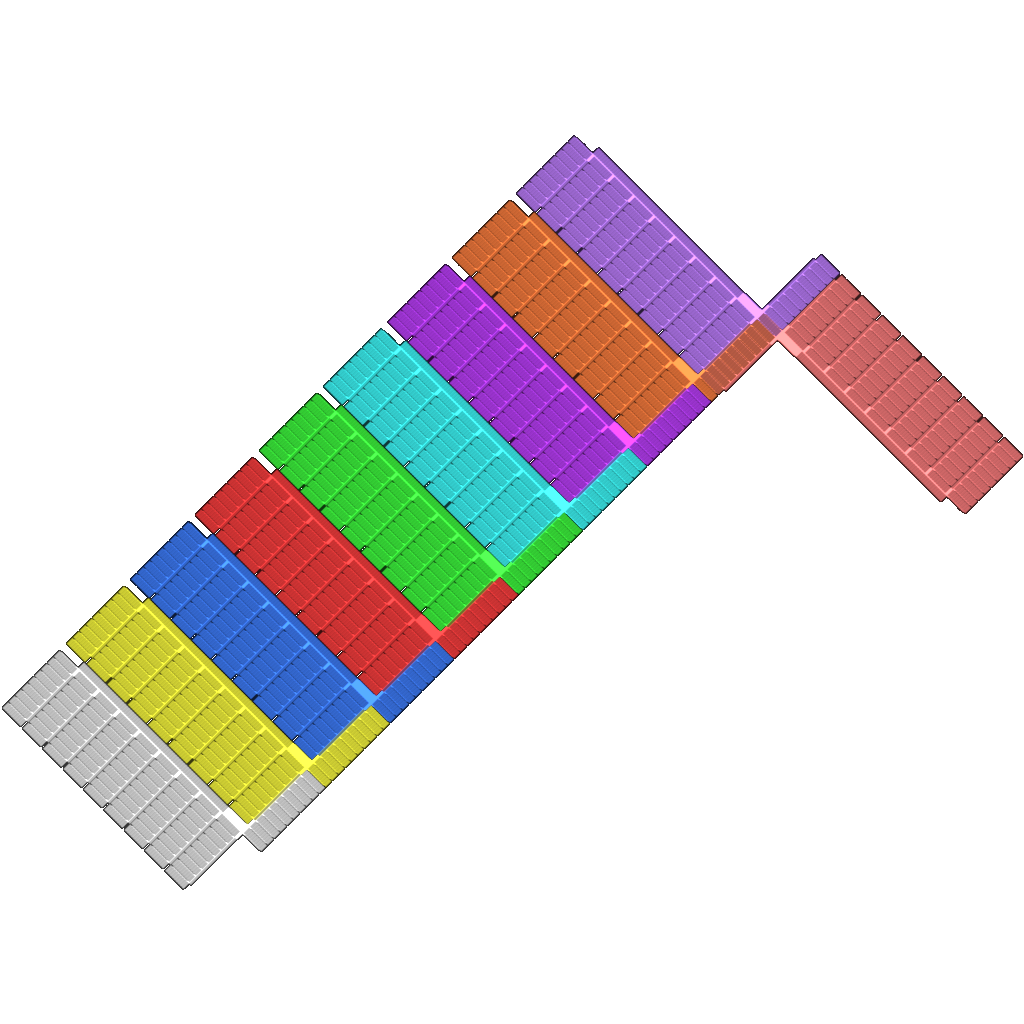
\includegraphics[width=0.48\textwidth]{comb-tile-n10.png}
\caption{Boundary complexity progression.
  \emph{Left:} the comb tile $A_3$ ($n = 3$, three maps),
  $\dH(\partial A_3) \approx 1.453$ --- the boundary is visibly
  fractal.
  \emph{Right:} the comb tile $A_{10}$ ($n = 10$, ten maps),
  $\dH(\partial A_{10}) \approx 1.973$ --- the boundary is nearly
  space-filling, and the tile is almost polygonal.
  Compare with~$A_5$ in Figure~\ref{fig:comb-tile}.}
\label{fig:comb-progression}
\end{figure}

Each contraction $f_j = g^{-1} \circ h_j$ is an affine similarity with
linear part $g^{-1}$ (for $j < n{-}1$) or $-g^{-1}$ (for $j = n{-}1$), and
common contraction ratio $1/\sqrt{n}$.

\begin{remark}[Digit set geometry]
\label{rem:digits}
The first $n{-}1$ digits $h_0, \ldots, h_{n-2}$ are pure translations
along the first coordinate axis, with displacements
$0,\, n{-}1,\, 2(n{-}1),\, \ldots,\, (n{-}2)(n{-}1)$.  These form the
\emph{spine} of the comb.
The single map $h_{n-1}$, which includes a central reflection, has an
off-axis translation component and forms the \emph{tooth} of the comb.
This asymmetric digit geometry --- one outlier map among $n{-}1$ collinear
ones --- is the structural source of the small neighbor graph size
(see Section~\ref{sec:osc}).
The name \emph{comb} reflects the first-level subdivision visible in
Figure~\ref{fig:comb-tile}: the $n{-}1$ spine pieces form a row of
teeth, while the single reflected piece extends sideways like a handle.
\end{remark}

\subsection{Basic properties}

Since all $n$ maps share the contraction ratio $r = 1/\sqrt{n}$, the
Hausdorff dimension of the attractor is
\[
  \dH(A_n) = \frac{\log n}{\log \sqrt{n}} = 2
\]
for every~$n$.  Thus each $A_n$ is a plane-filling set (a tile).

To verify the tiling property rigorously, we reformulate
{\cite[Theorem~2]{bandt1991}} in a form where the residue condition
is identical to the purely translational case (Theorem~1 ibid.).

\begin{proposition}[Tiling criterion with symmetries,
  after {\cite[Theorem~2]{bandt1991}}]
\label{prop:bandt-sym}
Let $g \in \Z^{d \times d}$ be expanding with $m = |\det g|$,
and let $P$ be a finite group of integer matrices with
$\det s = \pm 1$ for every $s \in P$, normalized by~$g$
(i.e.\ $gPg^{-1} = P$).
Given $s_1,\ldots,s_m \in P$ and
\emph{digit vectors} $h_1,\ldots,h_m \in \Z^d$,
define the attractor~$A$ by
\begin{equation}\label{eq:ifs-sym}
  A \;=\; \bigcup_{i=1}^{m} g^{-1}\,s_i(A + h_i).
\end{equation}
If $\{h_1,\ldots,h_m\}$ is a complete residue system
for $\Z^d / g\Z^d$, then $A$ has nonempty interior,
the open set condition holds with
$V = \operatorname{int}(A)$, and $\dH(A) = d$.
\end{proposition}

\begin{proof}
Set $y_i = s_i\,h_i$ and consider the contractions
$f_i(x) = s_i\,g^{-1}(x) + y_i$, which are in the
form of Theorem~2 in~\cite{bandt1991}.
The lattice condition of that theorem requires
\[
  \Z^d = \bigcup_{i=1}^{m} s_i^{-1}\bigl(y_i + g\Z^d\bigr).
\]
Since $gPg^{-1} = P$, we have
$g^{-1}s_i^{-1}g \in P \subset \mathrm{GL}(d,\Z)$, so
$s_i^{-1}\,g\Z^d = g(g^{-1}s_i^{-1}g)\Z^d = g\Z^d$, and
\[
  s_i^{-1}(y_i + g\Z^d)
  = s_i^{-1}y_i + g\Z^d
  = h_i + g\Z^d,
\]
and the condition reduces to $\{h_i\}$ being a complete
residue system for~$\Z^d/g\Z^d$ --- our hypothesis.

Theorem~2 of~\cite{bandt1991} now yields a unique attractor
$\hat{A} = \bigcup_i f_i(\hat{A})$ with nonempty interior and
$\dH(\hat{A}) = d$.
Setting $A = g^{-1}\hat{A}$, we verify~\eqref{eq:ifs-sym}:
\[
  g^{-1}\,s_i(A + h_i)
  = g^{-1}\bigl(s_i\,g^{-1}\hat{A} + s_i\,h_i\bigr)
  = g^{-1}\,f_i(\hat{A}),
\]
so $\bigcup g^{-1}\,s_i(A + h_i)
  = g^{-1}\hat{A} = A$.
Since $g^{-1}$ is a linear bijection,
$\operatorname{int}(A) \ne \emptyset$ and $\dH(A) = d$.
The open set condition
for~\eqref{eq:ifs-sym} holds with
$V = g^{-1}(\operatorname{int}\hat{A}) = \operatorname{int}(A)$.
\end{proof}

\begin{proposition}[Self-replicating tiling]\label{prop:tiling}
For every $n \ge 3$, $A_n$ is an $n$-rep tile in the sense
of~\cite{bandt1991}: the plane is tiled by copies of~$A_n$ and its
half-turn~$-A_n$:
\[
  \R^2 = \bigcup_{v \in \Z^2} (A_n + v)
         \;\cup\; \bigcup_{w \in \Z^2} (-A_n + w),
\]
with the union measure-disjoint.
\end{proposition}

\begin{proof}
The comb IFS (Definition~\ref{def:comb}) has the
form~\eqref{eq:ifs-sym} with $d = 2$, $P = \{I, -I\}$,
$s_j = I$ for $j < n{-}1$, and $s_{n-1} = -I$.
The digit vectors are
$h_j = j(n{-}1)\,e_1$ ($j = 0,\ldots,n{-}2$)
and $h_{n-1} = -\bigl(n^2{-}n{-}1,\;2n{-}3\bigr)$.
The companion matrix $g = C(x^2 - n)$ satisfies $|\det g| = n$
and $g\Z^2 = \{(ny, x) : x,y \in \Z\}$, so
$\Z^2/g\Z^2 \cong \Z/n\Z$ via the first coordinate modulo~$n$.
The first coordinates of the digit vectors modulo~$n$ are
$j(n{-}1) \equiv -j$ for $j < n{-}1$ and
$-(n^2{-}n{-}1) \equiv 1$ for $j = n{-}1$,
giving $\{0, n{-}1, n{-}2, \ldots, 1\}$, a complete
residue system.
Proposition~\ref{prop:bandt-sym} gives
$\operatorname{int}(A_n) \ne \emptyset$ and $\dH(A_n) = 2$.
The tiling by $\Z^2$-translates of $A_n$ and $-A_n$
follows from the neighbor graph (Theorem~\ref{thm:graph}).
\end{proof}

Following~\cite{bandt1991}, the maps above are written in~$\R^2$
with the integer lattice~$\Z^2$, so that $g$ and all digits have
integer entries.  Since $g$ has two real eigenvalues $\pm\sqrt{n}$
with independent eigenvectors, one can choose a basis in which $g$
acts as a Euclidean similarity, making the IFS self-similar
(rather than merely self-affine).

\begin{remark}[Complex form of the IFS]
\label{rem:eigenbasis}
Identify the eigenplane of~$g$ with~$\C$ by mapping the eigenvectors
for~$\sqrt{n}$ and~$-\sqrt{n}$ to the real and imaginary axes,
respectively.  Then the expansion acts as
\[
  g(z) = \sqrt{n}\,\bar{z},
\]
an anti-conformal map of modulus~$\sqrt{n}$.  Since
$g^{-1}(z) = \bar{z}/\sqrt{n}$, the IFS takes the form
\begin{equation}\label{eq:complex-ifs}
\begin{aligned}
  f_j(z) &= \frac{\bar{z}}{\sqrt{n}} + c_j,
    &\quad j &= 0,\ldots,n{-}2, \\[4pt]
  f_{n-1}(z) &= -\,\frac{\bar{z}}{\sqrt{n}} + c_{n-1},
\end{aligned}
\end{equation}
where the spine translations are uniformly spaced along
$\R \cdot (1{+}i)$:
\[
  c_j = \frac{j(n{-}1)(1{+}i)}{2n},
  \qquad j = 0,\ldots,n{-}2,
\]
and the tooth translation is
\[
  c_{n-1} = \frac{(n^2{-}n{-}1)(1{+}i)
             + (2n{-}3)\sqrt{n}\,(1{-}i)}{2n}.
\]
All maps are anti-conformal similarities of ratio
$1/\sqrt{n}$.  The spine digits are rational, but the
tooth digit involves~$\sqrt{n}$.
The rational-space representation of Definition~\ref{def:comb},
where \emph{all} digits are integer vectors, is therefore preferred
for the exact neighbor graph analysis in Section~\ref{sec:osc}.
\end{remark}

\begin{remark}[The case $n = 2$]
\label{rem:n2}
For $n = 2$ the attractor $A_2$ is a rectangle (a non-fractal,
disk-like tile).  The quartic~\eqref{eq:quartic} gives
$p_2(x) = x(x{-}1)(x^2{-}2)$ with dominant root~$\sqrt{2}$ and
$\dH(\partial A_2) = 1$, correctly matching the boundary dimension.
However, the neighbor graph has $8$~components (not~$6$), so the
specific graph structure and substitution matrix derived below
apply only to $n \ge 3$.
\end{remark}

% --------------------------------------------------------------------------
\section{The Neighbor Graph}
\label{sec:osc}

In this section we derive the neighbor graph of the comb IFS from first
principles, proving that it has exactly $6$~boundary components for every
$n \ge 3$.

\subsection{Neighbor map algebra}

A \emph{neighbor map} of the tile $A = A_n$ is an isometry
$\sigma \colon \R^2 \to \R^2$ such that $A \cap \sigma(A) \ne \emptyset$
and $\sigma \ne \mathrm{id}$~\cite{bandt1991,scheicher-thuswaldner}.  Because every contraction
$f_j = g^{-1} \circ h_j$ has linear part $\pm g^{-1}$, every neighbor
map has the form $\sigma(x) = \varepsilon x + t$ with
$\varepsilon \in \{+I, -I\}$ and $t \in \R^2$.

The \emph{refinement rule}: substituting $A = \bigcup_i f_i(A)$ into
both sides of $A \cap \sigma(A)$ gives
\[
  A \cap \sigma(A)
  = \bigcup_{i,j} f_i\bigl(A \cap \sigma'_{ij}(A)\bigr),
  \qquad
  \sigma'_{ij} = f_i^{-1} \circ \sigma \circ f_j.
\]
A direct calculation yields
\begin{equation}\label{eq:child}
  \sigma'_{ij}(x)
  = \varepsilon_i\varepsilon\varepsilon_j\, x
  + \varepsilon_i(\varepsilon\, d_j + g\,t - d_i),
\end{equation}
where $\varepsilon_j, d_j$ are the sign and digit of $h_j$.

The neighbor graph is the minimal set of neighbor types closed under
refinement~\eqref{eq:child} that is reachable from the identity.
A vertex $\sigma$ is an \emph{actual neighbor} if and only if the
directed graph of children~\eqref{eq:child} admits an infinite path
starting from $\sigma$~\cite{lau-ngai}.

\subsection{Invariant bounding set}

\begin{lemma}[Bounding rectangle]\label{lem:bound}
For every $n \ge 3$, the attractor satisfies
$A_n \subset R$, where
\begin{equation}\label{eq:bound-R}
  R = [0,\, 2n{-}3] \times [0,\, n{-}1{-}1/n].
\end{equation}
\end{lemma}

\begin{proof}
Write $R_0 = [0, 2n{-}3]^2$.  A direct computation shows
$\bigcup_j f_j(R_0) \subset R_0$, so $A \subset R_0$ by
Hutchinson's theorem.  Applying one Hutchinson step to $R_0$:
\begin{itemize}
\item Each spine piece $f_j(R_0)$, $0 \le j \le n{-}2$, satisfies
  $x_2 \le \bigl(2n{-}3 + (n{-}2)(n{-}1)\bigr)/n
  = (n^2{-}n{-}1)/n = n{-}1{-}1/n$.
\item The tooth piece $f_{n-1}(R_0)$ satisfies
  $x_2 \le (n^2{-}n{-}1)/n = n{-}1{-}1/n$.
\end{itemize}
Thus the overall $x_2$-range of $\bigcup f_j(R_0)$ is $[0,\, n{-}1{-}1/n]$.
The $x_1$-range remains $[0, 2n{-}3]$ (unchanged by the spine
and tooth strips).  A second Hutchinson step verifies that
$R = [0, 2n{-}3] \times [0, n{-}1{-}1/n]$ is invariant.
\end{proof}

We also record the \emph{refined bound}
$A \subset B_1 = \bigcup_j f_j(R)$, which decomposes into rectangular
strips:
\begin{equation}\label{eq:B1-strips}
\begin{aligned}
  \text{spine strip:}\quad & x_1 \in [0,\, n{-}1{-}1/n], \quad
    x_2 \in [0,\, (n^2{-}3n{+}5)/n], \\
  \text{tooth strip:}\quad & x_1 \in [n{-}2{+}1/n,\, 2n{-}3], \quad
    x_2 \in [(n{-}1)(n{-}2)/n,\, n{-}1{-}1/n].
\end{aligned}
\end{equation}
In particular, points with $x_1 \ge n{-}1$ lie exclusively in the
tooth strip.

\subsection{Level-1 neighbors}

\begin{proposition}[Level-1 neighbors]\label{prop:level1}
The children of the identity under~\eqref{eq:child} that satisfy
$A \cap \sigma(A) \ne \emptyset$ are precisely:
\begin{alignat*}{2}
  \sigma_1 &= (+I,\; (n{-}1,\, 0)),
    &\qquad& \text{spine, forward}, \\
  \sigma_2 &= (+I,\; (-(n{-}1),\, 0)),
    &\qquad& \text{spine, backward}, \\
  \sigma_3 &= (-I,\; (3n{-}4,\, 2n{-}3)),
    &\qquad& \text{spine--tooth, far}, \\
  \sigma_4 &= (-I,\; (2n{-}3,\, 2n{-}3)),
    &\qquad& \text{spine--tooth, near}.
\end{alignat*}
\end{proposition}

\begin{proof}
The children of the identity are $\sigma_{ij} = f_i^{-1} f_j$
with $i \ne j$.  By~\eqref{eq:child},
$\sigma_{ij}(x) = \varepsilon_i\varepsilon_j\, x
  + \varepsilon_i(d_j - d_i)$.

\emph{Spine--spine} ($i, j \le n{-}2$): the sign is $+I$ and the
translation is $((j{-}i)(n{-}1),\, 0)$.
For overlap, $A \cap (A + t) \ne \emptyset$ requires
$|t_1| \le \mathrm{width}_{x_1}(A) \le 2n{-}3$.  Thus
$|j{-}i|\,(n{-}1) \le 2n{-}3$, giving $|j{-}i| \le 1$ (since
$(2n{-}3)/(n{-}1) = 2 - 1/(n{-}1) < 2$).  This yields
$\sigma_1$ and $\sigma_2$.

\emph{Spine--tooth} ($i \le n{-}2,\; j = n{-}1$ or vice versa):
the sign is $-I$ and the translation is
$d_{n-1} - d_i = \bigl((n{-}1)(n{-}i) - 1,\; 2n{-}3\bigr)$.
For overlap with sign $-I$, the translation must lie in
$A + A \subset [0,\, 2(2n{-}3)] \times [0,\, 2(n{-}1{-}1/n)]$.
The $x_1$-constraint gives $(n{-}1)(n{-}i) - 1 \le 4n{-}6$,
hence $n{-}i \le (4n{-}5)/(n{-}1) < 4$, so $i \ge n{-}3$.
This yields $\sigma_3$ (from $i = n{-}3$) and $\sigma_4$ (from
$i = n{-}2$).

All other candidates are infeasible by the $R$-bound.
\end{proof}

\subsection{Level-2 neighbors and graph closure}

\begin{theorem}[Neighbor graph]\label{thm:graph}
For every integer $n \ge 3$, the neighbor graph of the comb IFS consists
of exactly $6$ neighbor types $\sigma_1, \ldots, \sigma_6$, where
$\sigma_1, \ldots, \sigma_4$ are as above and
\begin{alignat*}{2}
  \sigma_5 &= (-I,\; (2n{-}3,\, n{-}2)),
    &\qquad& \text{level-2, diagonal}, \\
  \sigma_6 &= (-I,\; (n{-}2,\, n{-}2)),
    &\qquad& \text{level-2, reflected}.
\end{alignat*}
In particular, the Open Set Condition holds for all $n \ge 3$
(and trivially for $n = 2$, where $A_2$ is a rectangle).
\end{theorem}

\begin{proof}
We compute the children~\eqref{eq:child} of $\sigma_1, \ldots, \sigma_4$,
identify the new types $\sigma_5, \sigma_6$, verify graph closure, and
eliminate one spurious candidate~$\tau$.

\emph{Step~1: Children of $\sigma_1$ and $\sigma_2$.}
For $\sigma_1 = (+I, (n{-}1, 0))$, the ``$gt$'' vector is
$g(n{-}1, 0) = (0, n{-}1)$.  The spine--spine children have
sign~$+I$ and translation $((k{-}j)(n{-}1),\; n{-}1)$.  Since
$n{-}1 > n{-}1{-}1/n = \mathrm{height}(R)$, the $x_2$-component
exceeds the diameter of $A{-}A$ in the $x_2$-direction: all
spine--spine children are infeasible.

The only surviving child comes from the tooth--spine case
$(i, j) = (n{-}1,\, n{-}2)$, which produces
$\sigma_5 = (-I, (2n{-}3, n{-}2))$ via the map~$f_{n-1}$.
By symmetry, $\sigma_2$ also produces $\sigma_5$ (via~$f_{n-2}$).

\emph{Step~2: Children of $\sigma_3$.}
The only surviving child is from $(i, j) = (n{-}1, n{-}1)$
(tooth--tooth), producing $\sigma_6 = (-I, (n{-}2, n{-}2))$
via~$f_{n-1}$.

\emph{Step~3: Children of $\sigma_4$.}
The surviving children are:
\begin{itemize}
\item $(i, j) = (n{-}2,\, n{-}1)$: $\sigma_1$, via $f_{n-2}$;
\item $(i, j) = (n{-}1,\, n{-}2)$: $\sigma_2$, via $f_{n-1}$;
\item $(i, j) = (n{-}2,\, n{-}2)$: $\sigma_3$, via $f_{n-2}$;
\item $(i, j) = (n{-}1,\, n{-}1)$: $\tau = (-I, (n{-}2, 2n{-}3))$,
via $f_{n-1}$.
\end{itemize}
The candidate $\tau$ is not among the six types; we handle it below.

\emph{Step~4: Children of $\sigma_5$.}
The spine--spine children $f_i^{-1} \sigma_5 f_j$ with
$i, j \le n{-}2$ have sign~$-I$ and translation
$\bigl((n{-}1)(n{-}1{-}i{-}j) - 1,\; 2n{-}3\bigr)$.
Among these:
\begin{itemize}
\item $i + j = n{-}4$: produces $\sigma_3$
  ($n{-}3$~ways, maps $f_0, \ldots, f_{n-4}$);
\item $i + j = n{-}3$: produces $\sigma_4$
  ($n{-}2$~ways, maps $f_0, \ldots, f_{n-3}$);
\item $i + j = n{-}2$: produces $\tau$
  ($n{-}1$~ways); handled below.
\end{itemize}
The tooth--spine child $(i, j) = (n{-}1,\, 0)$ gives $\sigma_1$
via $f_{n-1}$, and the spine--tooth child $(i, j) = (0,\, n{-}1)$
gives~$\sigma_2$ via~$f_0$.
All other children are infeasible.

\emph{Step~5: Children of $\sigma_6$.}
The spine--spine children have sign~$-I$ and translation
$\bigl((n{-}1)(n{-}1{-}i{-}j) - 1,\; n{-}2\bigr)$:
\begin{itemize}
\item $i + j = n{-}3$: produces $\sigma_5$
  ($n{-}2$~ways, maps $f_0, \ldots, f_{n-3}$);
\item $i + j = n{-}2$: produces $\sigma_6$
  ($n{-}1$~ways, maps $f_0, \ldots, f_{n-2}$).
\end{itemize}
All other children of $\sigma_6$ are infeasible (by the $R$-bound or
the $B_1$ refinement).

\emph{Step~6: Elimination of $\tau = (-I, (n{-}2, 2n{-}3))$.}
The candidate $\tau$ passes the coarse bounding-box test, so we must
refine further.  Among all $n^2$~children of $\tau$, only one is
feasible by the $R$-bound: the spine--spine child
$(i, j) = (n{-}2,\, n{-}2)$, which produces
$\tau' = (-I, (3n{-}4,\, n{-}2))$.

We eliminate $\tau'$ using the refined bound~$B_1$.  For
$A \cap \tau'(A) \ne \emptyset$ with sign $-I$, we need
$p + q = (3n{-}4,\, n{-}2)$ for some $p, q \in A$.
Since $p_1 + q_1 = 3n{-}4$ and $\max(x_1) = 2n{-}3$, both
$p_1 \ge n{-}1$ and $q_1 \ge n{-}1$.  By~\eqref{eq:B1-strips},
points with $x_1 \ge n{-}1$ lie in the \emph{tooth strip}, where
$x_2 \ge (n{-}1)(n{-}2)/n$.  Therefore
\[
  p_2 + q_2 \;\ge\; \frac{2(n{-}1)(n{-}2)}{n},
\]
but the target is $p_2 + q_2 = n{-}2$.  The inequality
$2(n{-}1)(n{-}2)/n \le n{-}2$ simplifies to $2(n{-}1)/n \le 1$,
i.e., $n \le 2$, contradicting $n \ge 3$.
Thus $\tau'$ is infeasible, so $\tau$ has no infinite path in the
refinement graph and is not an actual neighbor.

\emph{Conclusion.}
Since $\sigma_5$ and $\sigma_6$ produce only children from
$\{{\rm id}, \sigma_1, \ldots, \sigma_6\}$ (plus the eliminated
$\tau$), the graph is closed.  Every vertex $\sigma_k$ admits an
infinite path: the cycle
$\sigma_1 \to \sigma_5 \to \sigma_4 \to \sigma_1$ (and analogously
for the others) ensures $A \cap \sigma_k(A) \ne \emptyset$.
The finiteness of the neighbor graph implies the OSC~\cite{lau-ngai}.
\end{proof}

\begin{remark}[Neighbor count]
\label{rem:neighbor-count}
Each of the six neighbor types $\sigma_1, \ldots, \sigma_6$ corresponds
to exactly one adjacent tile in the tiling, so every copy of~$A_n$ has
precisely $6$~neighbors.  This is the minimum possible for a disk-like
tile that tiles the plane: by Euler's formula for normal planar
tilings~\cite[Section~3.3]{grunbaum-shephard},
the average number of neighbors is at least~$6$, with equality
corresponding to the hexagonal combinatorics.  The comb family thus
achieves this topological minimum despite the extreme geometric
complexity of the boundary ($\dH(\partial A_n) \to 2$).
\end{remark}

\begin{remark}
For $n = 3$ the general formulas specialise: the $B_3$-contribution
to $B_5$ in~\eqref{eq:bnd-rules} is an empty union (since
$n - 4 < 0$), reflecting the fact that at $n = 3$ no pair
$(i,j) \in \{0,\ldots,n{-}2\}^2$ satisfies $i + j = n{-}4 = -1$.
The $B_4$-contribution collapses from $n{-}2$ distinct maps to a
single map $f_0 = f_{n-3}$.
\end{remark}

\subsection{Boundary substitution rules}

The proof of Theorem~\ref{thm:graph} determines the boundary GIFS
explicitly.  Writing $B_k = A \cap \sigma_k(A)$ for the six
boundary pieces and reading off which map $f_i$ produces each
child, we obtain the substitution rules (valid for all $n \ge 3$):
\begin{equation}\label{eq:bnd-rules}
\begin{aligned}
  B_1 &= f_{n-1}(B_5), \\
  B_2 &= f_{n-2}(B_5), \\
  B_3 &= f_{n-1}(B_6), \\
  B_4 &= f_{n-2}(B_1) \cup f_{n-2}(B_3) \cup f_{n-1}(B_2), \\
  B_5 &= f_{n-1}(B_1) \cup f_0(B_2)
    \cup \bigcup_{j=0}^{n-4} f_j(B_3)
    \cup \bigcup_{j=0}^{n-3} f_j(B_4), \\
  B_6 &= \bigcup_{j=0}^{n-3} f_j(B_5 \cup B_6) \cup f_{n-2}(B_6).
\end{aligned}
\end{equation}
The $6 \times 6$ substitution (count) matrix $M_n$, with $(M_n)_{jk}$
equal to the number of occurrences of $B_k$ on the right-hand side of
the rule for~$B_j$, is:
\begin{equation}\label{eq:subst-matrix}
  M_n =
  \begin{pmatrix}
    0 & 0 & 0 & 0 & 1 & 0 \\
    0 & 0 & 0 & 0 & 1 & 0 \\
    0 & 0 & 0 & 0 & 0 & 1 \\
    1 & 1 & 1 & 0 & 0 & 0 \\
    1 & 1 & n{-}3 & n{-}2 & 0 & 0 \\
    0 & 0 &   0 &   0 & n{-}2 & n{-}1
  \end{pmatrix}.
\end{equation}

\begin{figure}[ht]
\centering
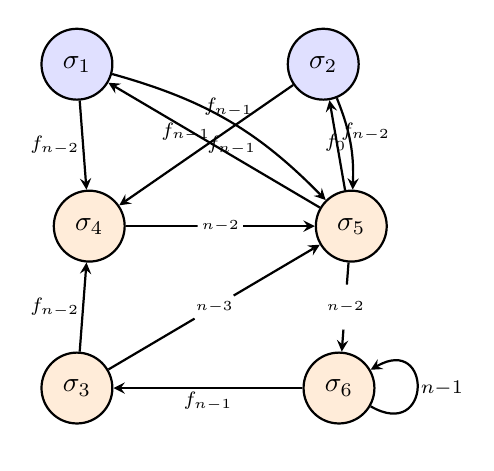
\begin{tikzpicture}[
  node distance=2.2cm,
  vtx/.style={circle, draw, thick, minimum size=9mm, inner sep=0pt},
  spine/.style={vtx, fill=blue!12},
  tooth/.style={vtx, fill=orange!15},
  arr/.style={-stealth, thick},
  lbl/.style={font=\scriptsize, inner sep=1pt},
  mlbl/.style={font=\scriptsize, inner sep=1pt, fill=white, circle},
]
  % Nodes
  \node[spine] (s1) {$\sigma_1$};
  \node[spine, right=2.2cm of s1] (s2) {$\sigma_2$};
  \node[tooth, below right=1.4cm and -0.5cm of s1] (s4) {$\sigma_4$};
  \node[tooth, right=2.4cm of s4] (s5) {$\sigma_5$};
  \node[tooth, below left=1.4cm and -0.5cm of s4] (s3) {$\sigma_3$};
  \node[tooth, right=2.4cm of s3] (s6) {$\sigma_6$};

  % Multiplicity-1 edges with map labels
  \draw[arr] (s5) -- node[lbl, above left]  {$f_{n-1}$} (s1);
  \draw[arr] (s5) -- node[lbl, above right] {$f_{n-2}$} (s2);
  \draw[arr] (s6) -- node[lbl, below]       {$f_{n-1}$} (s3);
  \draw[arr] (s1) -- node[lbl, left]        {$f_{n-2}$} (s4);
  \draw[arr] (s2) -- node[lbl, right=-1pt]  {$f_{n-1}$} (s4);
  \draw[arr] (s3) -- node[lbl, left]        {$f_{n-2}$} (s4);
  \draw[arr] (s1) to[bend left=15] node[lbl, above] {$f_{n-1}$} (s5);
  \draw[arr] (s2) to[bend left=12] node[lbl, left]  {$f_0$}     (s5);

  % Multiplicity >1 edges with count labels
  \draw[arr] (s3) -- node[mlbl] {{\tiny$n{-}3$}} (s5);
  \draw[arr] (s4) -- node[mlbl] {{\tiny$n{-}2$}} (s5);
  \draw[arr] (s5) -- node[mlbl] {{\tiny$n{-}2$}} (s6);
  \draw[arr] (s6) to[out=-30, in=30, looseness=5]
    node[lbl, right] {$n{-}1$} (s6);
\end{tikzpicture}
\caption{The boundary substitution graph of the comb IFS.  Vertices are
  the $6$~neighbor types: $\sigma_1, \sigma_2$ (spine--spine,
  sign~$+I$; shaded blue) and $\sigma_3, \ldots, \sigma_6$
  (spine--tooth or level-2, sign~$-I$; shaded orange).  A directed
  edge $\sigma_k \to \sigma_j$ means that the boundary piece~$B_k$
  contributes to~$B_j$ under substitution~\eqref{eq:bnd-rules}.
  Edges of multiplicity~$1$ are labelled with the producing map~$f_i$;
  edges of higher multiplicity show the count.
  The graph topology is independent of~$n$ (for $n \ge 3$); only the
  multiplicities depend on~$n$.}
\label{fig:neighbor-graph}
\end{figure}

% --------------------------------------------------------------------------
\section{Disk-Like Property}
\label{sec:disklike}

A self-similar tile $A$ is called \emph{disk-like} if it is homeomorphic to the
closed unit disk; see~\cite{bandt-wang,leung-lau} for criteria
and~\cite{akiyama-thuswaldner,ngai-tang} for surveys.  As noted in the Introduction, tiles with large
$\dH(\partial A)$ are generically non-disk-like, so achieving
$\dH(\partial A)$ close to~$2$ while maintaining the disk-like property
is particularly challenging.

The comb tiling is not a lattice tiling: the tooth map $f_{n-1}$ has
linear part~$-I$, so tiles related by~$f_{n-1}$ differ by a
$180^\circ$~rotation.  The tiling $\{A + d : d \in \Z^2\}$ must
therefore be replaced by a \emph{crystallographic tiling}
$\{\gamma(A) : \gamma \in \Gamma\}$, where $\Gamma$ is a discrete
cocompact group of isometries (a \emph{crystallographic group}).
For the comb family, $\Gamma$ is the ornament group~$p2$, generated by
two lattice translations and a $180^\circ$ rotation~$\rho$.
A compact set~$T$ satisfying a set equation of the form
$g(T) = \bigcup_{\delta \in D} \delta(T)$, where $g$ is an expanding
map and $D \subset \Gamma$ is a finite digit set, is called a
\emph{crystallographic reptile} (or \emph{crystile}) with respect
to~$\Gamma$~\cite[Definition~1]{loridant-luo-thuswaldner}.

For such a tiling, the \emph{neighbor set}
$S = \{\gamma \in \Gamma \setminus \{{\rm id}\} : T \cap \gamma(T)
\ne \emptyset\}$
and the \emph{boundary pieces}
$B_\gamma = T \cap \gamma(T)$ for $\gamma \in S$
are defined as before.  A neighbor $\gamma$ is an
\emph{edge neighbor} if $B_\gamma$ contains a point of the interior
of $T \cup \gamma(T)$; a neighbor is a \emph{vertex neighbor} if
$B_\gamma$ is a single point.  The set of edge neighbors is denoted
$\mathcal{A} \subseteq S$.

Two further graphs encode how boundary pieces meet after one
substitution step.  The \emph{double neighboring graph}~$G_2$ has
vertices $\{B_\gamma : \gamma \in S\}$, with an edge between
$B_{\gamma_1}$ and $B_{\gamma_2}$ whenever they intersect
($\gamma_1 \ne \gamma_2$).
For each $\gamma \in \mathcal{A}$, the \emph{boundary piece
graph}~$G_\gamma$ is the subgraph of~$G_2$ on the set of sub-pieces
\[
  V_\gamma \;=\;
  \bigl\{\, \delta\bigl(B_{\delta^{-1} g\gamma g^{-1}\delta'}\bigr)
  \;:\; \delta, \delta' \in D,\;
  \delta^{-1} g\gamma g^{-1}\delta' \in \mathcal{A} \,\bigr\};
\]
these are the images of boundary pieces that constitute
$g(B_\gamma)$ under the set
equation~\cite[Definition~4]{loridant-luo-thuswaldner}.
In our notation, with digits $f_i(x) = g^{-1}(\varepsilon_i x + d_i)$
and neighbors $\sigma_k = (\varepsilon_k, t_k)$, the vertices
of~$G_{\sigma_k}$ are exactly the sub-pieces $f_i(B_{\sigma_\ell})$
appearing on the right-hand side of the boundary substitution
rule~\eqref{eq:bnd-rules} for~$B_k$.

\begin{theorem}[{\cite[Theorem~4.2]{loridant-luo-thuswaldner}}]%
\label{thm:disklike-criterion}
Let $T \subset \R^2$ be a crystallographic reptile with respect
to~$\Gamma$, with expanding map~$g$ and digit set~$D$.
Let $S$ denote the set of neighbors and $\mathcal{A} \subseteq S$ the
subset of edge neighbors.  Then $T$~is disk-like if and only if:
\begin{enumerate}
\item[\rm(1)] for every pair of distinct $\gamma_1, \gamma_2 \in S$,
  the triple intersection
  $T \cap \gamma_1(T) \cap \gamma_2(T)$ is empty or a single point;
\item[\rm(2)] for each $\gamma \in \mathcal{A}$, the graph $G_\gamma$
  consists of a simple path;
\item[\rm(3)] the subgraph of~$G_2$ with
  vertices $\{B_\gamma : \gamma \in \mathcal{A}\}$ is a simple loop.
\end{enumerate}
\end{theorem}

We verify all three conditions for the comb family.

\begin{lemma}[Double neighboring graph — condition~(3)]%
\label{lem:simple-loop}
For every $n \ge 3$, the double neighboring graph $G_2$ restricted to
the six edge neighbors $\sigma_1, \ldots, \sigma_6$ is the cycle
\[
  B_1 - B_3 - B_4 - B_2 - B_6 - B_5 - B_1.
\]
\end{lemma}

\begin{proof}
Two boundary pieces $B_j$ and $B_k$ ($j \ne k$) are connected by an
edge in $G_2$ if and only if $\sigma_j^{-1} \circ \sigma_k$ is a
neighbor, i.e., belongs to $\{\sigma_1, \ldots, \sigma_6\}$.

For $\sigma_j = (\varepsilon_j, t_j)$ and $\sigma_k = (\varepsilon_k, t_k)$,
the composition $\sigma_j^{-1} \circ \sigma_k$ has sign
$\varepsilon_j \varepsilon_k$ and translation
$\varepsilon_j(t_k - t_j)$.  We check all $\binom{6}{2} = 15$ pairs.
Writing $t_j$ for the translation vector of $\sigma_j$, the six
translations are:
\[
\begin{aligned}
  t_1 &= (n{-}1,\, 0), &\quad
  t_2 &= (-(n{-}1),\, 0), \\
  t_3 &= (3n{-}4,\, 2n{-}3), &\quad
  t_4 &= (2n{-}3,\, 2n{-}3), \\
  t_5 &= (2n{-}3,\, n{-}2), &\quad
  t_6 &= (n{-}2,\, n{-}2).
\end{aligned}
\]
The signs are $\varepsilon_1 = \varepsilon_2 = +I$,\;
$\varepsilon_3 = \varepsilon_4 = \varepsilon_5 = \varepsilon_6 = -I$.
Since $\varepsilon_j \varepsilon_k = +I$ when the signs are equal and
$-I$ when they differ, we compare $\varepsilon_j(t_k - t_j)$
with the known neighbor translations (and signs) to identify which
pairs are edges in~$G_2$.

The $6$~pairs that yield a neighbor $\sigma_\ell$ are:
\begin{alignat*}{3}
  &(1,3):&\quad &\sigma_1^{-1}\sigma_3 = (-I,\; t_3 - t_1) = \sigma_4,\\
  &(1,5):&\quad &\sigma_1^{-1}\sigma_5 = (-I,\; t_5 - t_1) = \sigma_6,\\
  &(2,4):&\quad &\sigma_2^{-1}\sigma_4 = (-I,\; t_4 - t_2) = \sigma_3,\\
  &(2,6):&\quad &\sigma_2^{-1}\sigma_6 = (-I,\; t_6 - t_2) = \sigma_5,\\
  &(3,4):&\quad &\sigma_3^{-1}\sigma_4 = (+I,\; -(t_4 - t_3)) = \sigma_1,\\
  &(5,6):&\quad &\sigma_5^{-1}\sigma_6 = (+I,\; -(t_6 - t_5)) = \sigma_1.
\end{alignat*}
The remaining $9$~pairs produce translations outside the set of
neighbor translations (a routine but straightforward check; for
instance, $\sigma_1^{-1}\sigma_2$ has translation $(-(2n{-}2),0)$,
which exceeds the bounding-box diameter for $n \ge 3$).

The edges of $G_2$ are therefore $B_1 B_3$,\; $B_1 B_5$,\; $B_2 B_4$,\;
$B_2 B_6$,\; $B_3 B_4$,\; $B_5 B_6$.\;  Each vertex has degree~$2$,
and the graph is the $6$-cycle
$B_1 - B_3 - B_4 - B_2 - B_6 - B_5 - B_1$.
\end{proof}

\begin{figure}[ht]
\centering
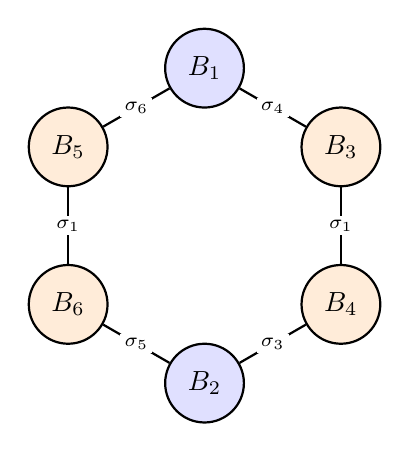
\begin{tikzpicture}[
  bvtx/.style={circle, draw, thick, minimum size=10mm, inner sep=0pt},
  bspine/.style={bvtx, fill=blue!12},
  btooth/.style={bvtx, fill=orange!15},
  elbl/.style={font=\scriptsize, fill=white, inner sep=1.5pt},
]
  % Vertices on a regular hexagon (clockwise: B1, B3, B4, B2, B6, B5)
  \node[bspine] (B1) at ( 90:2cm) {$B_1$};
  \node[btooth] (B3) at ( 30:2cm) {$B_3$};
  \node[btooth] (B4) at (330:2cm) {$B_4$};
  \node[bspine] (B2) at (270:2cm) {$B_2$};
  \node[btooth] (B6) at (210:2cm) {$B_6$};
  \node[btooth] (B5) at (150:2cm) {$B_5$};

  % Edges with mediating-neighbor labels
  \draw[thick] (B1) -- node[elbl]         {$\sigma_4$} (B3);
  \draw[thick] (B3) -- node[elbl]         {$\sigma_1$} (B4);
  \draw[thick] (B4) -- node[elbl]         {$\sigma_3$} (B2);
  \draw[thick] (B2) -- node[elbl]         {$\sigma_5$} (B6);
  \draw[thick] (B6) -- node[elbl]         {$\sigma_1$} (B5);
  \draw[thick] (B5) -- node[elbl]         {$\sigma_6$} (B1);
\end{tikzpicture}
\caption{The double neighboring graph~$G_2$ for the comb family
  (Lemma~\ref{lem:simple-loop}).  The six boundary pieces form a
  hexagonal cycle.  Edge labels indicate the mediating neighbor:
  $B_j$--$B_k$ is an edge when
  $\sigma_j^{-1}\sigma_k = \sigma_\ell \in \mathcal{A}$.
  Spine-type pieces $B_1, B_2$ are shaded blue; tooth-type pieces
  $B_3, \ldots, B_6$ orange.  Note that $\sigma_1$ appears on two
  opposite edges ($B_3 B_4$ and $B_5 B_6$): it is the cross-map
  link that connects consecutive spine maps in the
  graphs~$G_{\sigma_5}$ and~$G_{\sigma_6}$.}
\label{fig:g2-cycle}
\end{figure}

\begin{lemma}[Boundary piece graphs --- condition~(2)]%
\label{lem:simple-path}
For every $n \ge 3$ and every edge neighbor $\gamma \in \{\sigma_1,
\ldots, \sigma_6\}$, the graph $G_\gamma$ is a simple path.
\end{lemma}

\begin{proof}
The graph $G_\gamma$ has one vertex for each sub-piece appearing
in the boundary substitution rule~\eqref{eq:bnd-rules} for~$B_\gamma$,
and an edge between two sub-pieces when they are pairwise neighbors at
the next refinement level.  We verify the path structure for each
boundary piece.

\emph{Case $B_1$, $B_2$, $B_3$.}
The rules $B_1 = f_{n-1}(B_5)$,\; $B_2 = f_{n-2}(B_5)$,\;
$B_3 = f_{n-1}(B_6)$ each contain a single sub-piece.  A graph on one
vertex is a (trivial) simple path.

\emph{Case $B_4$.}
The rule is $B_4 = f_{n-2}(B_1) \cup f_{n-2}(B_3) \cup f_{n-1}(B_2)$.
We check adjacency of the three sub-pieces.  Two sub-pieces
$f_i(B_j)$ and $f_k(B_\ell)$ are neighbors if $f_i^{-1}\sigma_4 f_k$
composed with the neighbor data of $B_j, B_\ell$ yields a neighbor.
Since $f_{n-2}$ and $f_{n-1}$ are adjacent maps (their level-1
neighbor is $\sigma_4$), and both $B_1$ and $B_3$ touch $B_2$
in the cyclic order of~$G_2$ (Lemma~\ref{lem:simple-loop}), the
three sub-pieces form a path:
$f_{n-2}(B_1) - f_{n-2}(B_3) - f_{n-1}(B_2)$.

\emph{Case $B_5$.}
The rule~\eqref{eq:bnd-rules} gives $2n{-}3$ sub-pieces.  For $n \ge 4$
these are
\[
  f_0(B_2),\; f_0(B_4),\; f_0(B_3),\;
  f_1(B_4),\; f_1(B_3),\; \ldots,\;
  f_{n-4}(B_4),\; f_{n-4}(B_3),\;
  f_{n-3}(B_4),\; f_{n-1}(B_1);
\]
for $n = 3$ the $B_3$-union in~\eqref{eq:bnd-rules} is empty and the
three sub-pieces are $f_0(B_2),\, f_0(B_4),\, f_2(B_1)$.
Two sub-pieces from the \emph{same} map~$f_j$ are adjacent in~$G_{\sigma_5}$
when the corresponding boundary pieces are adjacent in~$G_2$.
Since $B_2 B_4$ and $B_3 B_4$ are edges of~$G_2$
(Lemma~\ref{lem:simple-loop}) but $B_2 B_3$ is not,
the three sub-pieces from~$f_0$ form the path
$f_0(B_2) - f_0(B_4) - f_0(B_3)$.

For \emph{cross-map} adjacency between $f_j$ and $f_{j+1}$
($j, j{+}1 \le n{-}2$), the level-1 neighbor is
$\sigma_1 = f_j^{-1} f_{j+1}$.
A sub-piece $f_j(B_\alpha)$ intersects $f_{j+1}(B_\beta)$ only
if $B_\alpha$ meets~$B_1$ and $B_\beta$ meets~$B_2$ in~$G_2$.
Among the available indices, only $B_3$ is adjacent to~$B_1$ and
only $B_4$ is adjacent to~$B_2$, so the unique cross-map edge is
$f_j(B_3) - f_{j+1}(B_4)$.

The last transition from $f_{n-3}(B_4)$ to $f_{n-1}(B_1)$ uses
$\sigma_3 = f_{n-3}^{-1}f_{n-1}$: we need $B_4$ adjacent to~$B_3$
and $B_1$ adjacent to~$B_3$ in~$G_2$, both of which hold.

No non-consecutive sub-pieces are adjacent: maps $f_j, f_\ell$ with
$|j - \ell| \ge 2$ have tiles of $x_1$-diameter at most $2n{-}3$
separated by distance $(n{-}1)|j - \ell| - (2n{-}3) > 0$.
Hence the path is (for $n \ge 4$):
\begin{align*}
  &f_0(B_2) - f_0(B_4) - f_0(B_3) - f_1(B_4) - f_1(B_3) - \cdots\\
  &\quad\cdots - f_{n-4}(B_3) - f_{n-3}(B_4) - f_{n-1}(B_1),
\end{align*}
while for $n = 3$ it degenerates to
$f_0(B_2) - f_0(B_4) - f_2(B_1)$, with the last edge via
$\sigma_3 = f_0^{-1} f_2$.
In all cases $G_{\sigma_5}$ is a simple path on $2n{-}3$ vertices.

\emph{Case $B_6$.}
The rule gives $2n{-}3$ sub-pieces:
\[
  f_0(B_6),\; f_0(B_5),\; f_1(B_6),\; f_1(B_5),\;
  \ldots,\; f_{n-3}(B_6),\; f_{n-3}(B_5),\; f_{n-2}(B_6).
\]
Within each~$f_j$, the sub-pieces $f_j(B_5)$ and $f_j(B_6)$ are
adjacent ($B_5 B_6$ is an edge of~$G_2$).
For the cross-map adjacency via $\sigma_1 = f_j^{-1}f_{j+1}$:
among $\{B_5, B_6\}$, only $B_5$ is adjacent to~$B_1$ and only
$B_6$ is adjacent to~$B_2$ in~$G_2$, so the unique cross-map edge
is $f_j(B_5) - f_{j+1}(B_6)$.
No non-consecutive sub-pieces are neighbors (same separation argument).
Hence $G_{\sigma_6}$ is the simple path
\[
  f_0(B_6) - f_0(B_5) - f_1(B_6) - f_1(B_5) - \cdots
  - f_{n-3}(B_5) - f_{n-2}(B_6).
  \qedhere
\]
\end{proof}

\begin{figure}[ht]
\centering
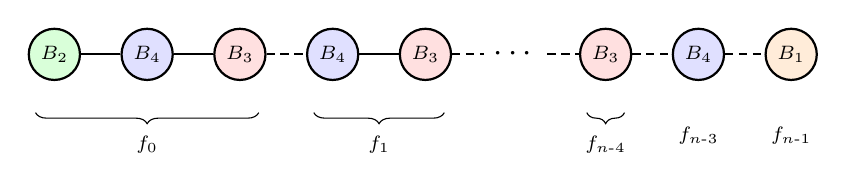
\begin{tikzpicture}[
  pnode/.style={circle, draw, thick, minimum size=6.5mm, inner sep=0pt,
                font=\scriptsize},
  p2/.style={pnode, fill=green!15},
  p4/.style={pnode, fill=blue!12},
  p3/.style={pnode, fill=red!12},
  p1/.style={pnode, fill=orange!15},
  intra/.style={thick},
  cross/.style={thick, densely dashed},
  maplbl/.style={font=\scriptsize, below=3pt},
]
  % Row of nodes for the G_{sigma_5} path (general n)
  \node[p2]                  (v1) {$B_2$};
  \node[p4, right=5mm of v1] (v2) {$B_4$};
  \node[p3, right=5mm of v2] (v3) {$B_3$};
  \node[p4, right=5mm of v3] (v4) {$B_4$};
  \node[p3, right=5mm of v4] (v5) {$B_3$};
  \node[right=4mm of v5, font=\large] (dots) {$\cdots$};
  \node[p3, right=4mm of dots] (v6) {$B_3$};
  \node[p4, right=5mm of v6] (v7) {$B_4$};
  \node[p1, right=5mm of v7] (v8) {$B_1$};

  % Intra-map edges (solid)
  \draw[intra] (v1) -- (v2);
  \draw[intra] (v2) -- (v3);
  \draw[intra] (v4) -- (v5);

  % Cross-map edges (dashed)
  \draw[cross] (v3) -- (v4);
  \draw[cross] (v5) -- (dots);
  \draw[cross] (dots) -- (v6);
  \draw[cross] (v6) -- (v7);
  \draw[cross] (v7) -- (v8);

  % Map-index braces
  \draw[decorate, decoration={brace, mirror, amplitude=4pt}]
    ([yshift=-5mm]v1.south west) -- ([yshift=-5mm]v3.south east)
    node[midway, below=5pt, font=\scriptsize] {$f_0$};
  \draw[decorate, decoration={brace, mirror, amplitude=4pt}]
    ([yshift=-5mm]v4.south west) -- ([yshift=-5mm]v5.south east)
    node[midway, below=5pt, font=\scriptsize] {$f_1$};
  \draw[decorate, decoration={brace, mirror, amplitude=4pt}]
    ([yshift=-5mm]v6.south west) -- ([yshift=-5mm]v6.south east)
    node[midway, below=5pt, font=\scriptsize] {$f_{n\text{-}4}$};
  \node[font=\scriptsize, below=8mm] at (v7) {$f_{n\text{-}3}$};
  \node[font=\scriptsize, below=8mm] at (v8) {$f_{n\text{-}1}$};
\end{tikzpicture}
\caption{The boundary piece graph $G_{\sigma_5}$ for the
  comb family (Lemma~\ref{lem:simple-path}, Case~$B_5$).
  Solid edges connect sub-pieces within the same
  map~$f_j$ (adjacency in~$G_2$); dashed edges connect
  sub-pieces from consecutive maps $f_j, f_{j+1}$ via the
  cross-map neighbor~$\sigma_1$.  Each cross-map link is uniquely
  determined: $B_3$ is the only sub-piece adjacent to~$B_1$, and
  $B_4$ the only one adjacent to~$B_2$ in~$G_2$
  (Figure~\ref{fig:g2-cycle}), so the edge must be
  $f_j(B_3)$--$f_{j+1}(B_4)$.  The graph is a simple path on
  $2n{-}3$ vertices.}
\label{fig:g-sigma5}
\end{figure}

\begin{theorem}[Disk-like]\label{thm:disklike}
For every integer $n \ge 2$, the comb tile $A_n$ is disk-like.
\end{theorem}

\begin{proof}
For $n = 2$, the attractor $A_2$ is a rectangle, so the claim is
trivial.  For $n \ge 3$, conditions~(2) and~(3) of
Theorem~\ref{thm:disklike-criterion} are established in
Lemmas~\ref{lem:simple-path} and~\ref{lem:simple-loop}; it remains to
verify condition~(1).  We identify the first-level intersection graph,
show it has a unique triangle, and prove the corresponding triple
intersection is a single point.

\emph{Step~1: First-level intersection graph.}
Two first-level tiles $f_i(A)$ and $f_j(A)$ intersect if and only if
$f_i^{-1} \circ f_j$ is a neighbor.
By Proposition~\ref{prop:level1}, the only neighbors arising as
children of the identity are $\sigma_1, \ldots, \sigma_4$.  These
correspond to the pairs:
\begin{itemize}
\item Spine consecutive: $(j,\, j{+}1)$ for $j = 0, \ldots, n{-}3$,
  giving $\sigma_1$ (or its inverse $\sigma_2$);
\item Tooth: $(n{-}3,\, n{-}1)$ giving $\sigma_3$, and
  $(n{-}2,\, n{-}1)$ giving $\sigma_4$.
\end{itemize}
The resulting graph is a path $0 {-} 1 {-} \cdots {-} (n{-}2)$ with
vertex~$n{-}1$ adjacent to $n{-}3$ and~$n{-}2$.  Its only clique of
size~$3$ is $\{n{-}3,\; n{-}2,\; n{-}1\}$.

\emph{Step~2: Triple refinement is unique.}
Write $T = f_{n-3}(A) \cap f_{n-2}(A) \cap f_{n-1}(A)$ for the
unique triple intersection.  Substituting $A = \bigcup_k f_k(A)$,
\[
  T = \bigcup_{\substack{a,b,c \\ \text{pairwise}\\\text{feasible}}}
  f_{n-3} \circ f_a(A) \;\cap\;
  f_{n-2} \circ f_b(A) \;\cap\;
  f_{n-1} \circ f_c(A),
\]
where a triple $(a, b, c)$ is \emph{pairwise feasible} if
$f_a^{-1} \sigma_1 f_b$,\; $f_b^{-1} \sigma_4 f_c$,\;
$f_a^{-1} \sigma_3 f_c$ are all neighbors.
Here $\sigma_1 = f_{n-3}^{-1} f_{n-2}$,
$\sigma_4 = f_{n-2}^{-1} f_{n-1}$,
$\sigma_3 = f_{n-3}^{-1} f_{n-1}$ are the three pairwise neighbor
maps of the triangle.

The key observation: $\sigma_1$ and $\sigma_2$ each have exactly
\emph{one} surviving child under refinement~\eqref{eq:child}.
For~$\sigma_1 = (+I, (n{-}1, 0))$, the vector $gt = g \cdot (n{-}1, 0) =
(0,\, n{-}1)$.  All spine--spine children
$f_\alpha^{-1} \sigma_1 f_\beta$ (with $\alpha, \beta \le n{-}2$)
have translation component
$t_2' = n{-}1 > n{-}1{-}1/n = \mathrm{height}(R)$,
so they exceed the $R$-bound
and are infeasible.  We check the three remaining child types
(those involving the tooth index $n{-}1$):
\begin{itemize}
\item \emph{Spine--tooth} ($\alpha \le n{-}2$, $j = n{-}1$):
  sign~$-I$, translation $\bigl((n{-}1)(n{-}\alpha)-1,\; 3n{-}4\bigr)$.
  The $x_2$-component $3n{-}4$ exceeds the sum
  $2 \cdot \mathrm{height}(R) = 2(n{-}1{-}1/n)$ for $n \ge 3$,
  so $A \cap \sigma(A) = \emptyset$ for all~$\alpha$.
\item \emph{Tooth--tooth} ($\alpha = j = n{-}1$):
  sign~$+I$, translation $(0,\,{-}(n{-}1))$.
  This requires $x_2 \ge n{-}1$ in~$A$, but
  $A \subset R$ has $x_2 \le n{-}1{-}1/n$; infeasible.
\item \emph{Tooth--spine} ($\alpha = n{-}1$, $\beta \le n{-}2$):
  sign~$-I$, translation $\bigl((n{-}1)(n{-}\beta)-1,\; n{-}2\bigr)$.
  For $\beta \le n{-}3$ the first component
  $(n{-}1)(n{-}\beta)-1 \ge 3n{-}4$, forcing both summands in the
  $A + A$ representation into the tooth strip
  ($x_1 \ge n{-}1$, hence $x_2 \ge (n{-}1)(n{-}2)/n$
  by~\eqref{eq:B1-strips}); then
  $p_2 + q_2 \ge 2(n{-}1)(n{-}2)/n > n{-}2$ for $n \ge 3$,
  contradicting $p_2 + q_2 = n{-}2$.
  Only $\beta = n{-}2$ survives, giving translation $(2n{-}3,\,n{-}2)$.
\end{itemize}
Thus the unique surviving child is
\[
  f_{n-1}^{-1} \circ \sigma_1 \circ f_{n-2} = \sigma_5,
\]
which fixes $a = n{-}1$ and $b = n{-}2$.

With $a = n{-}1$ fixed, we evaluate the children of~$\sigma_3$
at $(n{-}1,\, c)$.  For spine indices $c \le n{-}2$, the
translation has $|t_2'| = n{-}1 > \mathrm{height}(R)$ (infeasible),
while for $c = n{-}1$ the child is
\[
  f_{n-1}^{-1} \circ \sigma_3 \circ f_{n-1} = \sigma_6.
\]
This forces $c = n{-}1$.  A consistency check confirms
$f_{n-2}^{-1} \circ \sigma_4 \circ f_{n-1} = \sigma_1$.
Thus the unique refinement triple is $(a, b, c) = (n{-}1, n{-}2,
n{-}1)$, and the new pairwise state is $(\sigma_5,\, \sigma_1,\,
\sigma_6)$.

\emph{Step~3: Period-$2$ cycle.}
Iterating the same analysis for the state
$(\sigma_5,\, \sigma_1,\, \sigma_6)$:
\begin{itemize}
\item $\sigma_1$ (the ``bottleneck'') again forces $b = n{-}1$,
  $c = n{-}2$, giving $\sigma_5$.
\item For $\sigma_5$, the child $f_\alpha^{-1} \sigma_5 f_{n-1}$
  with spine~$\alpha$ has translation
  $t_1' = -(n{-}1)(1{+}\alpha)$.  Only $\alpha = 0$ yields
  $|t_1'| = n{-}1 \le 2n{-}3$, giving $\sigma_2$.  So $a = 0$.
\item $f_0^{-1} \circ \sigma_6 \circ f_{n-2} = \sigma_6$ (since
  $0 + (n{-}2) = n{-}2$).
\end{itemize}
The new state is $(\sigma_2,\, \sigma_5,\, \sigma_6)$.

One more iteration (using $\sigma_2$, which has the same
bottleneck property as $\sigma_1$, giving a unique child $\sigma_5$
at $(a, b) = (n{-}2,\, n{-}1)$) returns to the state
$(\sigma_5,\, \sigma_1,\, \sigma_6)$.

The refinement thus cycles with period~$2$:
\[
  (\sigma_5, \sigma_1, \sigma_6)
  \;\longrightarrow\;
  (\sigma_2, \sigma_5, \sigma_6)
  \;\longrightarrow\;
  (\sigma_5, \sigma_1, \sigma_6)
  \;\longrightarrow\; \cdots
\]
At each level, the triple intersection is covered by a single
level-$k$ tile of diameter $O(n^{-k/2})$.  As $k \to \infty$,
the nested compact sets converge to a single point.

By Theorem~\ref{thm:disklike-criterion}\,(1), every triple
intersection is a single point.  Condition~(2) holds by
Lemma~\ref{lem:simple-path}, and condition~(3) by
Lemma~\ref{lem:simple-loop}.  Hence $A_n$ is disk-like for all
$n \ge 3$ (and hence for all $n \ge 2$).
\end{proof}

\begin{figure}[ht]
\centering
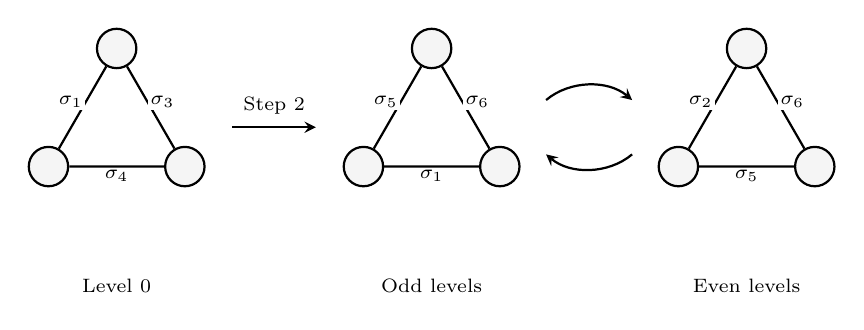
\begin{tikzpicture}[
  tv/.style={circle, draw, thick, minimum size=5mm, inner sep=0pt,
             font=\scriptsize, fill=gray!8},
  tlbl/.style={font=\scriptsize, fill=white, inner sep=1pt},
  trans/.style={-stealth, thick, shorten >=2pt, shorten <=2pt},
  cyc/.style={-stealth, thick, shorten >=2pt, shorten <=2pt,
              bend left=40},
  steplbl/.style={font=\scriptsize, above=1pt},
]
  % --- Triangle 0 (initial) ---
  \begin{scope}[shift={(0,0)}]
    \node[tv] (a0) at (90:1cm)  {};
    \node[tv] (b0) at (210:1cm) {};
    \node[tv] (c0) at (330:1cm) {};
    \draw[thick] (a0) -- node[tlbl, above right=-2pt] {$\sigma_3$} (c0)
                 -- node[tlbl, below]                  {$\sigma_4$} (b0)
                 -- node[tlbl, above left=-2pt]        {$\sigma_1$} (a0);
    \node[font=\scriptsize, below=13mm] at (0,-0.5) {Level $0$};
  \end{scope}

  % Arrow
  \draw[trans] (1.4,0) -- node[steplbl] {Step 2} (2.6,0);

  % --- Triangle 1 ---
  \begin{scope}[shift={(4,0)}]
    \node[tv] (a1) at (90:1cm)  {};
    \node[tv] (b1) at (210:1cm) {};
    \node[tv] (c1) at (330:1cm) {};
    \draw[thick] (a1) -- node[tlbl, above right=-2pt] {$\sigma_6$} (c1)
                 -- node[tlbl, below]                  {$\sigma_1$} (b1)
                 -- node[tlbl, above left=-2pt]        {$\sigma_5$} (a1);
    \node[font=\scriptsize, below=13mm] at (0,-0.5) {Odd levels};
  \end{scope}

  % Arrows for the period-2 cycle
  \draw[cyc] (5.4, 0.3) to node[steplbl, above=2pt] {} (6.6, 0.3);
  \draw[cyc] (6.6,-0.3) to node[steplbl, below=2pt] {} (5.4,-0.3);

  % --- Triangle 2 ---
  \begin{scope}[shift={(8,0)}]
    \node[tv] (a2) at (90:1cm)  {};
    \node[tv] (b2) at (210:1cm) {};
    \node[tv] (c2) at (330:1cm) {};
    \draw[thick] (a2) -- node[tlbl, above right=-2pt] {$\sigma_6$} (c2)
                 -- node[tlbl, below]                  {$\sigma_5$} (b2)
                 -- node[tlbl, above left=-2pt]        {$\sigma_2$} (a2);
    \node[font=\scriptsize, below=13mm] at (0,-0.5) {Even levels};
  \end{scope}
\end{tikzpicture}
\caption{Triple-point refinement (Theorem~\ref{thm:disklike},
  condition~(1)).  Each triangle shows the pairwise neighbor
  state of the three tiles meeting at the triple point.
  After one refinement (Step~2), the state enters a period-$2$
  cycle: the pair $\{\sigma_5, \sigma_6\}$ persists while the
  third edge alternates between $\sigma_1$ and~$\sigma_2$.
  Since each level nests inside a single tile of diameter
  $O(n^{-k/2})$, the triple intersection converges to a point.}
\label{fig:triple-refinement}
\end{figure}

\begin{remark}
Both the neighbor graph (Theorem~\ref{thm:graph}) and the disk-like
property (Theorem~\ref{thm:disklike}) are proved for all $n \ge 3$ by
the same structural argument: the combinatorial pattern of neighbors
and their children depends only on the relative positions of the
spine endpoint, the tooth, and their immediate predecessors,
not on the spine length.  Only the translations change with~$n$.
\end{remark}

\begin{remark}[Topological structure of $A_n$]
\label{rem:topology}
The disk-like property, together with the explicit structure of~$G_2$
and the boundary substitution~\eqref{eq:bnd-rules}, yields a
complete topological description of the comb tiling.

\begin{enumerate}
\item \emph{Jordan boundary.}
Since $A_n$ is disk-like, $A_n \cong \overline{\mathbb{D}}$ and
$\partial A_n$ is a Jordan curve (by the Sch\"onflies theorem).

\item \emph{Six boundary arcs in cyclic order.}
The $G_2$-cycle
$B_1 \!-\! B_3 \!-\! B_4 \!-\! B_2 \!-\! B_6 \!-\! B_5 \!-\! B_1$
(Lemma~\ref{lem:simple-loop}) determines a decomposition of
$\partial A_n$ into six arcs, each of which is the common boundary
with one neighbor.  Adjacent arcs in the cycle meet at exactly one
point.

\item \emph{Six triple points.}
The six arc junctions are the only points where three or more tiles
meet (condition~(1) of Theorem~\ref{thm:disklike-criterion}).
Each such point has valence~$3$ in the tiling.

\item \emph{Hexagonal combinatorial type.}
Although $\dH(\partial A_n) \to 2$ as $n \to \infty$
(Theorem~\ref{thm:dim}), the combinatorics of the tiling is
independent of~$n$ and coincides with that of the regular hexagonal
tiling: every tile has exactly $6$ edge neighbors and $6$ vertices,
with vertex valence~$3$.

\item \emph{Self-similar arc structure.}
The substitution rules~\eqref{eq:bnd-rules} and the simple-path
property of the graphs $G_{\sigma_k}$
(Lemma~\ref{lem:simple-path}) imply that each boundary arc is an
IFS attractor in its own right: at every substitution step the
sub-pieces of each arc form a chain without branching or loops,
so the arc remains a topological arc at every scale.
\end{enumerate}
\end{remark}

% --------------------------------------------------------------------------
\section{Boundary Dimension}
\label{sec:dim}

\subsection{Derivation of the quartic}

\begin{theorem}[Boundary dimension formula]\label{thm:dim}
For every integer $n \ge 3$, the characteristic polynomial of $M_n$
factors as
\begin{equation}\label{eq:charpoly-factor}
  \det(\lambda I - M_n) = \lambda^2 \cdot p_n(\lambda),
\end{equation}
where $p_n$ is the quartic polynomial
\begin{equation}\label{eq:quartic}
  p_n(x) = x^4 - (n{-}1)\,x^3 - 2\,x^2 - (n{-}1)(n{-}4)\,x + n(n{-}2).
\end{equation}
The spectral radius $\lambda_n = \rho(M_n)$ is the unique root of $p_n$
in the interval $(n{-}1,\, n)$, and the boundary Hausdorff dimension is
\begin{equation}\label{eq:dim}
  \dH(\partial A_n) = \frac{2\log\lambda_n}{\log n}.
\end{equation}
\end{theorem}

\begin{proof}
The dimension formula~\eqref{eq:dim} follows from the
Mauldin--Williams theory~\cite{mauldin-williams} applied to the
boundary GIFS~\eqref{eq:bnd-rules}.  Since the original IFS
satisfies the OSC with $V = \operatorname{int}(A)$
(Theorem~\ref{thm:graph}), the boundary GIFS inherits the
hypotheses of~\cite{mauldin-williams};
see also~\cite{duvall-keesling-strichartz} for the same approach
applied to the boundaries of self-similar tiles.  All contractions
share the ratio $r = 1/\sqrt{n}$, so
$\dH(\partial A_n) = 2\log\rho(M_n)/\log n$.

To prove the factorisation~\eqref{eq:charpoly-factor}, we solve the
eigenvector equation $M_n v = \lambda v$ for $\lambda \ne 0$.
From the first three rows:
\[
  B_1 = B_2 = \frac{B_5}{\lambda}, \qquad
  B_3 = \frac{B_6}{\lambda}.
\]
Substituting into row~6:
$\lambda B_6 = (n{-}2) B_5 + (n{-}1) B_6$, whence
\begin{equation}\label{eq:B6-from-B5}
  B_6 = \frac{(n{-}2)\, B_5}{\lambda - (n{-}1)}.
\end{equation}
Substituting all of $B_1, B_2, B_3, B_6$ in terms of $B_5$ into row~4:
\[
  \lambda B_4 = \frac{2}{\lambda}\, B_5
    + \frac{(n{-}2)}{\lambda\bigl(\lambda-(n{-}1)\bigr)}\, B_5
  = \frac{B_5}{\lambda}\,\cdot\, \frac{2\lambda - n}{\lambda - (n{-}1)},
\]
giving
\begin{equation}\label{eq:B4-from-B5}
  B_4 = \frac{(2\lambda - n)\, B_5}
    {\lambda^2\bigl(\lambda - (n{-}1)\bigr)}.
\end{equation}
Finally, substituting into row~5:
\begin{align*}
  \lambda B_5 &= \frac{2}{\lambda}\, B_5
    + \frac{(n{-}3)(n{-}2)}{\lambda\bigl(\lambda-(n{-}1)\bigr)}\, B_5
    + \frac{(n{-}2)(2\lambda-n)}
      {\lambda^2\bigl(\lambda-(n{-}1)\bigr)}\, B_5.
\end{align*}
Dividing by $B_5 \ne 0$ and multiplying through by
$\lambda^2(\lambda-(n{-}1))$:
\begin{align*}
  \lambda^3\bigl(\lambda-(n{-}1)\bigr)
  &= 2\lambda\bigl(\lambda-(n{-}1)\bigr) \\
  &\quad + (n{-}3)(n{-}2)\lambda + (n{-}2)(2\lambda-n).
\end{align*}
Expanding and collecting terms, the right-hand side equals
$2\lambda^2 + (n{-}1)(n{-}4)\lambda - n(n{-}2)$, so we obtain
\[
  \lambda^4 - (n{-}1)\lambda^3 - 2\lambda^2
    - (n{-}1)(n{-}4)\lambda + n(n{-}2) = 0,
\]
which is $p_n(\lambda) = 0$.

The factor $\lambda^2$ accounts for the two zero eigenvalues arising from
the two linear dependencies in~$M_n$: the identical rows for $B_1$
and~$B_2$, and the relation
$(n{-}2) \cdot (\text{row } B_1) + (n{-}1) \cdot (\text{row } B_3)
 = \text{row } B_6$.
\end{proof}

\begin{remark}[Root location]
The polynomial $p_n$ satisfies:
\begin{alignat*}{2}
  p_n(n{-}1) &= -(n{-}2)(n^2{-}3n{+}1) &&< 0 \quad (n \ge 3), \\
  p_n(n)     &= 2n(2n{-}3)              &&> 0 \quad (n \ge 3),
\end{alignat*}
so the intermediate value theorem guarantees a root in $(n{-}1,\,n)$.
Uniqueness follows from Descartes' rule: the coefficients of $p_n$ exhibit
exactly two sign changes for $n \ge 3$, so $p_n$ has at most two positive
real roots; since a second root $\mu_n \in (1,n{-}1)$ is accounted for
separately (see Section~\ref{ssec:roots}), the root in $(n{-}1,n)$ is unique.
Since $p_n(0) = n(n{-}2) > 0$ for $n \ge 3$ and $p_n(1) = 2(n{-}2) > 0$,
there is also a root between $1$ and $n{-}1$; the dominant root is the
one in $(n{-}1,\,n)$.
\end{remark}

\subsection{Computed dimensions}

Table~\ref{tab:dims} lists the boundary dimension for selected values
of~$n$.

\begin{table}[h]
\centering
\caption{Boundary dimension of the comb tile $A_n$ for selected $n$.
The polynomial is $p_n(x)$ from~\eqref{eq:quartic}.}
\label{tab:dims}
\begin{tabular}{rccc}
\toprule
$n$ & $\lambda_n$ & $\dH(\partial A_n)$ & $2 - \dH(\partial A_n)$ \\
\midrule
  3 & 2.2213 & 1.4529 & 0.5471 \\
  4 & 3.3846 & 1.7590 & 0.2410 \\
  5 & 4.4790 & 1.8633 & 0.1367 \\
  6 & 5.5451 & 1.9120 & 0.0880 \\
  7 & 6.5951 & 1.9388 & 0.0612 \\
  8 & 7.6345 & 1.9550 & 0.0450 \\
  9 & 8.6665 & 1.9656 & 0.0344 \\
 10 & 9.6932 & 1.9729 & 0.0271 \\
 20 & 19.8279 & 1.9942 & 0.0058 \\
 50 & 49.9251 & 1.9992 & $7.67 \times 10^{-4}$ \\
100 & 99.9613 & 1.9998 & $1.68 \times 10^{-4}$ \\
\bottomrule
\end{tabular}
\end{table}

All numerical values in Tables~\ref{tab:dims} and~\ref{tab:ratio}
are computed from the dominant real root~$\lambda_n$ of the
explicit quartic~\eqref{eq:quartic} via the
formula~\eqref{eq:dim}; no numerical simulation of the IFS is
involved.

\subsection{Asymptotic expansion of the dominant root}

\begin{theorem}[Asymptotics]\label{thm:asymp}
The dominant root $\lambda_n$ of $p_n(x)$ satisfies
\begin{equation}\label{eq:lambda-asymp}
  \lambda_n = n - \frac{4}{n} + O\!\left(\frac{1}{n^2}\right)
  \qquad (n \to \infty).
\end{equation}
Consequently,
\begin{equation}\label{eq:dim-asymp}
  2 - \dH(\partial A_n) \;\sim\; \frac{8}{n^2\,\ln n}
  \qquad (n \to \infty).
\end{equation}
\end{theorem}

\begin{proof}
\emph{Step~1: Leading correction to $\lambda_n$.}
Write $x = n - u$ with $u = c_1/n + O(1/n^2)$.
Substituting into $p_n(x) = 0$ and collecting powers of~$n$, the
dominant balance at order $n^2$ gives
\[
  p_n\bigl(n - c_1/n\bigr)
  = (-c_1 + 4)\,n^2 + O(n).
\]
Setting the $n^2$ coefficient to zero yields $c_1 = 4$, hence
$\lambda_n = n - 4/n + O(1/n^2)$.

\emph{Verification of the $n^2$ balance.}
We expand each term of $p_n(x)$ with $x = n - c/n$:
\begin{align*}
  x^4 &= n^4 - 4cn^2 + 6c^2 + O(1/n^2), \\
  (n{-}1)\,x^3 &= n^4 - n^3 + 3cn^2 - 3cn + \cdots, \\
  2\,x^2 &= 2n^2 - 4c + O(1/n^2), \\
  (n{-}1)(n{-}4)\,x &= n^3 - 5n^2 + (4{-}c)\,n + O(1), \\
  n(n{-}2) &= n^2 - 2n.
\end{align*}
The $n^4$ and $n^3$ terms cancel exactly; the $n^2$ coefficient is
$-4c + 3c - 2 + 5 + 1 = -c + 4$, confirming $c = 4$.

\emph{Step~2: From $\lambda_n$ to $\dH(\partial A_n)$.}
With $\lambda_n = n\bigl(1 - 4/n^2 + O(1/n^3)\bigr)$, we have
\[
  \log\lambda_n = \log n + \log\!\bigl(1 - 4/n^2 + O(1/n^3)\bigr)
  = \log n - \frac{4}{n^2} + O\!\left(\frac{1}{n^3}\right).
\]
Therefore
\[
  \dH(\partial A_n) = \frac{2\log\lambda_n}{\log n}
  = 2 - \frac{8}{n^2\,\log n} + O\!\left(\frac{1}{n^3\,\log n}\right),
\]
which gives~\eqref{eq:dim-asymp}.  (Here $\log$ denotes the natural
logarithm.)
\end{proof}

\begin{remark}[Refined asymptotics]
The next term in the expansion of $\lambda_n$ can be extracted by the
same method: write $x = n - 4/n + c_2/n^2$ and substitute into
$p_n(x) = 0$.  The $n^2$~coefficient was already forced to zero by
$c_1 = 4$; balancing the coefficient of~$n$ (linear in~$c_2$) gives
$c_2 = 14$, so
\[
  \lambda_n = n - \frac{4}{n} + \frac{14}{n^2} + O(1/n^3).
\]
Substituting into $\dH(\partial A_n) = 2\log\lambda_n / \log n$ and
expanding, we obtain the refined gap formula
\[
  2 - \dH(\partial A_n)
  = \frac{8}{n^2\,\ln n}\left(1 - \frac{7}{2n} + O(1/n^2)\right).
\]
\end{remark}

\subsection{Numerical verification}

Table~\ref{tab:ratio} compares the exact gap $2 - \dH(\partial A_n)$
with the leading asymptotic $8/(n^2\,\ln n)$.  The ratio converges to~$1$
at the expected rate $1 - O(1/n)$.

\begin{table}[h]
\centering
\caption{Convergence of $(2 - \dH) \cdot n^2 \ln n / 8 \to 1$.}
\label{tab:ratio}
\begin{tabular}{rccl}
\toprule
$n$ & $2 - \dH(\partial A_n)$ & $8/(n^2\,\ln n)$ & Ratio \\
\midrule
   10 & $2.706 \times 10^{-2}$ & $3.474 \times 10^{-2}$ & 0.779 \\
   20 & $5.769 \times 10^{-3}$ & $6.679 \times 10^{-3}$ & 0.864 \\
   50 & $7.666 \times 10^{-4}$ & $8.177 \times 10^{-4}$ & 0.937 \\
  100 & $1.680 \times 10^{-4}$ & $1.737 \times 10^{-4}$ & 0.967 \\
  500 & $5.114 \times 10^{-6}$ & $5.148 \times 10^{-6}$ & 0.993 \\
 1000 & $1.154 \times 10^{-6}$ & $1.158 \times 10^{-6}$ & 0.997 \\
10000 & $8.683 \times 10^{-9}$ & $8.687 \times 10^{-9}$ & 1.000 \\
\bottomrule
\end{tabular}
\end{table}

\subsection{Root structure}
\label{ssec:roots}

The polynomial $p_n(x) = x^4 - (n{-}1)\,x^3 - 2\,x^2 - (n{-}1)(n{-}4)\,x + n(n{-}2)$
has the following properties for $n \ge 3$:

\begin{enumerate}
\item \textbf{Dominant root:} $\lambda_n \in (n{-}1,\, n)$, real and simple,
with $\lambda_n = n - 4/n + O(1/n^2)$.
\item \textbf{Second real root:} $\mu_n \in (1,\, n{-}1)$, with
$\mu_n = 1 + 2/n - 14/n^3 + O(1/n^4)$ (note that the $1/n^2$
coefficient vanishes).  Existence follows from $p_n(1) = 2(n{-}2) > 0$
and $p_n(n{-}1) = -(n{-}2)(n^2{-}3n{+}1) < 0$ for $n \ge 3$, by the
intermediate value theorem.
\item \textbf{Two remaining roots $\alpha_n, \beta_n$:} by Vieta's
relations,
\[
  \alpha_n + \beta_n = (n{-}1) - \lambda_n - \mu_n
                     = -2 + \frac{2}{n} + O(1/n^2),
\]
\[
  \alpha_n \beta_n = \frac{n(n{-}2)}{\lambda_n\, \mu_n}
                   = n - 4 + O(1/n).
\]
The pair is complex conjugate with common modulus
$|\alpha_n| = |\beta_n| = \sqrt{\alpha_n \beta_n} = \sqrt{n} - 2/\sqrt{n} + O(n^{-3/2})$.
\end{enumerate}

\begin{remark}[Coefficients as functions of $n$]
The coefficients of $p_n$ are polynomial in~$n$:
\[
  p_n(x) = x^4 - (n{-}1)\,x^3 - 2\,x^2 - (n^2{-}5n{+}4)\,x + (n^2{-}2n).
\]
In particular, the constant term $n^2 - 2n = n(n{-}2)$ is positive for
$n \ge 3$, and the linear coefficient $-(n^2{-}5n{+}4) =
-(n{-}1)(n{-}4)$ changes sign at $n = 4$.  For $n < 4$, the linear
coefficient is positive; for $n > 4$ it is negative.  This sign change
at $n = 4$ corresponds to a subtle shift in the boundary topology
(although the neighbor graph retains $6$~components throughout).
\end{remark}

\subsection{Spectral gap and monopole structure}
\label{ssec:spectral}

The substitution matrix~$M_n$ has characteristic polynomial
$x^2 \cdot p_n(x)$, so its nonzero eigenvalues are exactly the
four roots of the quartic.

\begin{definition}[Spectral gap]\label{def:spectral-gap}
Let $\lambda_1$ be the Perron eigenvalue of a boundary substitution
matrix and $|\lambda_2|$ the second-largest eigenvalue modulus.  The
\emph{spectral gap} is $\rho := |\lambda_2|/\lambda_1 \in [0,1)$.
We say the boundary GIFS is of \emph{monopole type} if
$\rho \ll 1$: the Perron eigenvector concentrates on a single
component, meaning one boundary piece dominates the asymptotic
iteration count while the remaining pieces contribute
exponentially less (their shares decay as~$\rho^k$ after $k$
substitution steps).
\end{definition}

For the comb family in the plane,
\[
  \rho_n = \frac{|\lambda_2|}{\lambda_n}
         = \frac{1}{\sqrt{n}} - \frac{2}{n^{3/2}} + O(n^{-5/2})
         \;\longrightarrow\; 0,
\]
so the boundary is of monopole type for every~$n \ge 3$, with
a spectral gap that improves monotonically.  This is a special
case of a dimension-independent phenomenon; see
\S\ref{ssec:monopole-d}.

\begin{remark}[Relative measures of boundary pieces]
\label{rem:measures}
The Perron eigenvector of~$M_n$ is proportional to the
$\mathcal{H}^s$-measure of each boundary piece.
Normalising $v_5 = 1$ and writing $\delta = \lambda_n - (n{-}1)$,
the eigenvector equations (from the proof of
Theorem~\ref{thm:dim}) give
\[
  v_1 = v_2 = \frac{1}{\lambda_n},\quad
  v_3 = \frac{n{-}2}{\lambda_n\,\delta},\quad
  v_4 = \frac{2\lambda_n - n}{\lambda_n^2\,\delta},\quad
  v_6 = \frac{n{-}2}{\delta}.
\]
Since $\lambda_n \to n$ and $\delta \to 1$, we obtain
$v_6 \sim n{-}2$ while $v_5 = 1$ and
$v_3 \approx 1$,
so $v_1 = v_2 \sim 1/n$ and $v_4 \sim 1/n$ are negligible.
The relative measures
$w_k = v_k / \sum_j v_j$ satisfy
\[
  w_6 \;\approx\; 1 - \frac{2}{n}, \qquad
  w_5 \;\approx\; w_3 \;\approx\; \frac{1}{n}, \qquad
  w_1 = w_2,\; w_4 = O(1/n^2).
\]
Thus, for large~$n$, the single piece~$B_6$ carries nearly all of the
$\mathcal{H}^s$-measure of~$\partial A_n$: it accounts for $46\%$
at $n = 3$, $82\%$ at $n = 10$, and $96\%$ at $n = 50$.
\end{remark}

% --------------------------------------------------------------------------
\section{Higher-Dimensional Generalization}
\label{sec:higherdim}

The comb construction extends naturally to all dimensions $d \ge 1$.
In this section we define the $d$-dimensional comb IFS, present exact
computational results for $d \le 7$, and formulate conjectures that
generalise the planar theory of
Sections~\ref{sec:osc}--\ref{sec:dim}.
The one-dimensional case $d = 1$ admits a closed-form analysis
and is treated separately in~\S\ref{ssec:d1};
it serves as a rigorous base case for the conjectures below.
All numerical results below were obtained by exact rational arithmetic
using IFStile~\cite{ifstile}; in particular, the neighbor graph
computations use no floating-point approximations.

\subsection{The $d$-dimensional comb IFS}

For integers $d \ge 1$ and $n \ge 3$, let
$g = C(x^d - n) \in \Z^{d \times d}$
be the companion matrix of $x^d - n$, with eigenvalues
$n^{1/d}\zeta_d^k$ ($k = 0, \ldots, d{-}1$,
$\zeta_d = e^{2\pi i/d}$) and spectral radius~$n^{1/d}$.
For $d = 1$ this reduces to the scalar $g = n$.

\begin{definition}[$d$-dimensional comb IFS]\label{def:comb-d}
The \emph{$d$-dimensional comb IFS} with parameters $d$ and~$n$ consists
of $n$ digit maps on~$\R^d$:
\begin{equation}\label{eq:comb-maps-d}
\begin{aligned}
  h_j(x) &= x + j(n{-}1)\,e_1,
    &\quad j &= 0, \ldots, n{-}2, \\[2pt]
  h_{n-1}(x) &= -x + \bigl(n^2{-}n{-}1,\;
    \underbrace{2n{-}3, \ldots, 2n{-}3}_{d-1}\bigr),
\end{aligned}
\end{equation}
where $e_1 = (1, 0, \ldots, 0)$
(for $d = 1$ the underbraced block is empty,
so $h_{n-1}(x) = -x + (n^2{-}n{-}1)$).
The attractor
$A_n^{(d)} = g^{-1}\bigl(\bigcup_{j=0}^{n-1} h_j(A_n^{(d)})\bigr)$.
\end{definition}

For $d = 2$ this recovers Definition~\ref{def:comb};
for $d = 1$, see~\S\ref{ssec:d1}.
The off-axis translation $2n{-}3 = 2(n{-}1) - 1$ is
the same in all $d{-}1$ transverse coordinates.

\begin{remark}[Motivation of the construction]
The construction of Definition~\ref{def:comb-d} was discovered by
a systematic IFStile~\cite{ifstile} search over self-similar IFS
minimising the number of boundary components, and its particular
form can be motivated from first principles only in part.
\begin{itemize}
\item \emph{Expansion.} Requiring $n$ digit maps of equal
  contraction ratio $n^{-1/d}$ and integer-matrix expansion
  forces, up to similarity, the companion matrix of a monic
  integer polynomial with constant term $\pm n$; the minimal
  such polynomial is $x^d - n$, used here.
\item \emph{Digit residues.} By Proposition~\ref{prop:bandt-sym},
  the digit set must project to a complete residue system modulo
  $g\Z^d \cong \Z/n\Z$.  Taking $n{-}1$ aligned digits at
  $0, n{-}1, 2(n{-}1), \ldots, (n{-}2)(n{-}1)$ along~$e_1$
  covers residues $\{0, -1, -2, \ldots, -(n{-}2)\}$
  (mod~$n$); a single additional digit with residue $\pm 1$
  completes the system for every~$n$ simultaneously, which
  explains why the same combinatorial pattern works for all $n$.
\item \emph{Transverse offset.} The specific value $2n{-}3$ of
  the transverse translation in $h_{n-1}$, as well as the choice
  of $-I$ rather than $+I$ for its linear part, were selected
  empirically to minimise the neighbor graph.  A first-principles
  derivation of these choices --- and a proof that the resulting
  graph complexity is the smallest possible in this
  expansion class --- remains open
  (see~\S\ref{sec:discussion}).
\end{itemize}
\end{remark}

We verify that $A_n^{(d)}$ is a tile by applying
Proposition~\ref{prop:bandt-sym} in dimension~$d$.

\begin{corollary}\label{cor:comb-tile}
For every $d \ge 1$ and $n \ge 3$, the attractor $A_n^{(d)}$
of Definition~\textup{\ref{def:comb-d}}
tiles~$\R^d$ and $\dH(A_n^{(d)}) = d$.
\end{corollary}

\begin{proof}
The symmetry group $P = \{I,-I\}$ centralizes every matrix.
The digit maps of Definition~\ref{def:comb-d} have the form
$h_j(x) = s_j\,x + d_j$ with $s_j = I$ for $j < n{-}1$
and $s_{n-1} = -I$.
Since $s_j(x + s_j^{-1}d_j) = s_j\,x + d_j$,
rewriting in the form~\eqref{eq:ifs-sym} gives digit vectors
$v_j = s_j^{-1}d_j$:
\[
  v_j = j(n{-}1)\,e_1 \;\;(j = 0,\ldots,n{-}2),
  \qquad
  v_{n-1} = -d_{n-1}.
\]
The companion matrix $g = C(x^d - n)$ satisfies $|\det g| = n$,
and $g\Z^d$ is spanned by $\{e_2,\ldots,e_d,\,ne_1\}$
(since $ge_k = e_{k+1}$ for $k < d$ and $ge_d = ne_1$),
so $\Z^d/g\Z^d \cong \Z/n\Z$ via the first coordinate modulo~$n$.
The first coordinates of the digit vectors modulo~$n$ are:
$j(n{-}1) \equiv -j$ for $j = 0,\ldots,n{-}2$,
and $-(n^2{-}n{-}1) \equiv 1$ for $j = n{-}1$.
Thus the residues are
$\{0, n{-}1, n{-}2, \ldots, 2, 1\} = \{0,1,\ldots,n{-}1\}$,
a complete system.
The result follows from Proposition~\ref{prop:bandt-sym}.
\end{proof}

\begin{remark}[Bounding parallelepiped]\label{rem:invariant-d}
The Hutchinson operator $F = \bigcup_j f_j$ maps the
\emph{$d$-dimensional comb box}
\[
  R_d \;=\; [0,\, 2n{-}3]^{d-1} \times [0,\, n{-}1{-}1/n]
\]
into itself: $F(R_d) \subseteq R_d$ for every $d \ge 1$ and
$n \ge 3$.  This generalises Lemma~\ref{lem:bound} ($d = 2$);
for $d = 1$ it gives the bounding interval
$R_1 = [0,\, n{-}1{-}1/n]$.
Indeed, $g^{-1}(y_1, \ldots, y_d) = (y_2, \ldots, y_d, y_1/n)$
(reducing to $g^{-1}(y) = y/n$ when $d = 1$),
so $g^{-1}(R_d) = [0,2n{-}3]^{d-2} \times [0, n{-}1{-}1/n]
\times [0, (2n{-}3)/n]$.  Adding the spine
translations $j(n{-}1)/n\cdot e_d$ ($j = 0, \ldots, n{-}2$)
fills the last coordinate of $R_d$ up to $(n^2{-}n{-}1)/n
= n{-}1{-}1/n$ and leaves the first $d{-}1$ coordinates inside
$R_d$.  The tooth piece $f_{n-1}(R_d)$ fits in the corner
$[0, 2n{-}3]^{d-2} \times [n{-}2{+}1/n,\, 2n{-}3]
\times [n{-}3{+}2/n,\, n{-}1{-}1/n]$
(the first interval is absent when $d \le 2$, the second when
$d = 1$).

Consequently $A_n^{(d)} = \bigcap_{k\ge 0} F^k(R_d)$ is a
monotone intersection of compact PL~sets.  This is the natural
starting point for any future ball-likeness proof
(see~\S\ref{sec:discussion}).
\end{remark}

Figure~\ref{fig:comb3d} shows the attractor $A_5^{(3)}$
in dimension $d = 3$.

\begin{figure}[h]
\centering
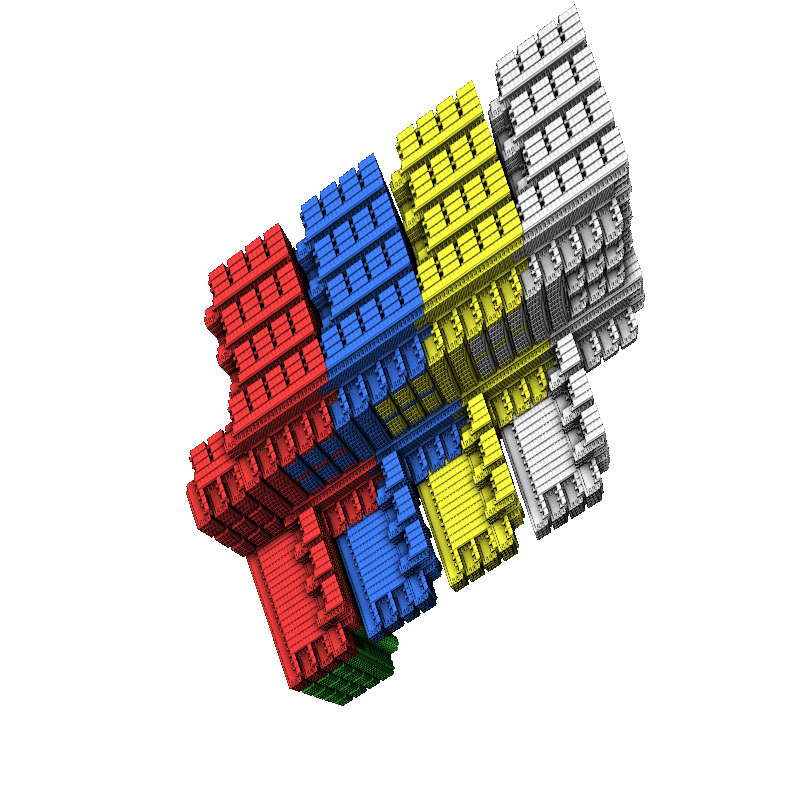
\includegraphics[width=0.5\textwidth]{comb3d_n5.png}
\caption{The $3$-dimensional comb tile $A_5^{(3)}$
  ($d = 3$, $n = 5$), rendered in the real Jordan basis of the
  companion matrix $g = C(x^3 - 5)$.}
\label{fig:comb3d}
\end{figure}

\begin{remark}[IFStile program for $d = 3$]\label{rem:aifs-3d}
The $3$-dimensional comb tile can be rendered in
IFStile~\cite{ifstile} using the following program
(shown for $n = 5$):
\begin{verbatim}
@
$dim=3
$subspace=[g,0,1]
g=$companion([-5,0,0])
h1=[4,0,0]
h2=[8,0,0]
h3=[12,0,0]
h4=[19,7,7]*-1
A=g^-1*(1|h1|h2|h3|h4)*A
\end{verbatim}
\noindent
Here \verb|$companion([-5,0,0])| creates the companion matrix
of $x^3 - 5$, and \verb|$subspace=[g,0,1]| projects
from~$\R^3$ to the eigenbasis of~$g$: the real eigenvalue
$5^{1/3}$ (index~$0$, one dimension) and the complex conjugate
pair $5^{1/3}\zeta_3^{\pm 1}$ (index~$1$, two dimensions).
For general $n \ge 3$, replace $-5$ with $-n$ in the companion
matrix, adjust the translations to
$h_j = [j(n{-}1),0,0]$ for $j = 1,\ldots,n{-}2$,
and set $h_{n-1} = [n^2{-}n{-}1,\; 2n{-}3,\; 2n{-}3] \cdot
(-I_3)$.
\end{remark}

\subsection{The closed-form case \texorpdfstring{$d = 1$}{d = 1}}
\label{ssec:d1}

Before stating the general conjectures, we analyse the
one-dimensional case in full.  Unlike the cases $d \ge 2$,
both the neighbor graph and the dominant root admit closed-form
expressions, providing a rigorous base case for the
conjectures formulated below.

At $d = 1$, Definition~\ref{def:comb-d} reads: scalar
expansion $g = n$ and digit maps
\[
  h_j(x) = x + j(n{-}1) \;\; (j = 0, \ldots, n{-}2), \qquad
  h_{n-1}(x) = -x + (n^2{-}n{-}1),
\]
so $f_j(x) = h_j(x)/n$ for $j < n{-}1$ and
$f_{n-1}(x) = (-x + n^2{-}n{-}1)/n$.  All contractions have
ratio $1/n$.

\begin{proposition}[Complete analysis at $d=1$]\label{prop:d1}
For every $n \ge 3$:
\begin{enumerate}
\item $A_n^{(1)}$ has positive Lebesgue measure and satisfies
  the OSC.
\item The neighbor graph has exactly two non-trivial types,
  \[
    \sigma_1(x) = -x + (2n{-}3), \qquad
    \sigma_2(x) = -x + (n{-}2).
  \]
\item The substitution matrix and its characteristic polynomial are
  \begin{equation}\label{eq:d1-matrix}
    M_n^{(1)} =
    \begin{pmatrix} 0 & 1 \\ n{-}2 & n{-}1 \end{pmatrix},
    \qquad
    q_n^{(1)}(x) = x^2 - (n{-}1)\,x - (n{-}2).
  \end{equation}
\end{enumerate}
\end{proposition}

\begin{proof}
\emph{Step 1 (OSC).}  The digits
$v_j = s_j^{-1} h_j(0) \bmod n$
form a complete residue system: for $j < n{-}1$ we have $s_j = I$
and $v_j = j(n{-}1) \equiv -j \pmod n$, while $s_{n-1} = -I$ and
$v_{n-1} = -(n^2{-}n{-}1) \equiv 1 \pmod n$, so
$\{v_0, \ldots, v_{n-1}\} \equiv \{0, 1, \ldots, n{-}1\} \pmod n$.
Proposition~\ref{prop:bandt-sym} now gives $\mu(A_n^{(1)}) > 0$
and the OSC.

\emph{Step 2 (bounding interval).}  Let
$L = (n^2{-}n{-}1)/n = n{-}1-1/n$ and $I = [0, L]$.  A direct
check shows $f_j(I) \subset I$ for every~$j$: for $j < n{-}1$ the
maximum of $f_j$ on $I$ is $(L + j(n{-}1))/n$, which at
$j = n{-}2$ equals $(n{-}1)^2 (2n{-}1) / (n^2(n{-}1))$ and is
bounded by~$L$ since $(n{-}1)^2 \ge 0$; for $f_{n-1}$ the
maximum is $(n^2{-}n{-}1)/n = L$.  Hence $A_n^{(1)} \subset I$.
Consequently, if $\sigma = f_i^{-1} f_j$ is a neighbor type
(i.e., $\sigma(A) \cap A \neq \emptyset$), its translation
component lies in $[-2L,\, 2L]$.

\emph{Step 3 (level-1 neighbors).}  Enumerate the ordered pairs
$(i, j)$ with $i \neq j$ by the orientations of $s_i$ and $s_j$:
\begin{itemize}
\item \emph{Both spine} ($i, j < n{-}1$):
  $\sigma(x) = x + (j{-}i)(n{-}1)$, translation
  $t = (j{-}i)(n{-}1)$ of modulus $\ge n{-}1$.  Since
  $n{-}1 > L$, the shifted interval $I + t$ intersects~$I$ only
  when $|t| < n{-}1-1/n$, which fails.  No contribution.
\item \emph{Tooth/spine} ($i = n{-}1$, $j < n{-}1$):
  $\sigma(x) = -x + t$ with
  $t = (n{-}1)(n{-}j) - 1$.  The admissibility
  $0 \le t \le 2L$ forces $n - j \le (2n{-}1)/(n{-}1) < 3$, i.e.,
  $j \in \{n{-}2, n{-}1\}$; excluding $j = n{-}1$ leaves $j = n{-}2$,
  $t = 2n{-}3$: the type $\sigma_1$.
\item \emph{Spine/tooth} ($i < n{-}1$, $j = n{-}1$): symmetric
  under $\sigma \mapsto \sigma^{-1}$ (and $\sigma_1^{-1} = \sigma_1$),
  giving the same type $\sigma_1$.
\end{itemize}
Level-1 thus yields a single type $\sigma_1$.

\emph{Step 4 (substitution row for $\sigma_1$).}  For each ordered
pair $(j, k)$ compute $\sigma' = f_j^{-1} \sigma_1 f_k$.
\begin{itemize}
\item $j, k < n{-}1$: $\sigma'(x) = -x + 2n^2 - 3n - (j+k)(n{-}1)$.
  Admissibility forces $j + k \ge 2n{-}3$, but
  $j + k \le 2(n{-}2) = 2n{-}4$; no contribution.
\item $j = n{-}1$ or $k = n{-}1$ (exactly one): $\sigma'$ is a
  translation $x \mapsto x \pm (n{-}1-m)(n{-}1)$ for
  $m \in \{0, \ldots, n{-}2\}$; the only admissible value is
  $\pm(n{-}1)$, and $A \pm (n{-}1)$ is disjoint from~$A$ (as
  in the spine/spine case).  No contribution.
\item $j = k = n{-}1$: $\sigma'(x) = -x + (n{-}2) = \sigma_2$.
  This is a new type, attached to $\sigma_1$ by a single edge.
\end{itemize}
This yields the first row $[0,\, 1]$ of $M_n^{(1)}$.

\emph{Step 5 (substitution row for $\sigma_2$).}  Similarly
decompose $\sigma'' = f_j^{-1} \sigma_2 f_k$.
\begin{itemize}
\item $j, k < n{-}1$: $\sigma''(x) = -x + n^2 - 2n - (j+k)(n{-}1)$,
  admissible iff $n{-}3 \le j + k \le n{-}2$.
  \begin{itemize}
    \item $j + k = n{-}3$: $t = 2n{-}3 = \sigma_1$,
          attained by $n{-}2$ pairs.
    \item $j + k = n{-}2$: $t = n{-}2 = \sigma_2$,
          attained by $n{-}1$ pairs.
  \end{itemize}
\item $j = n{-}1$ or $k = n{-}1$ (exactly one): $\sigma''$ is a
  translation whose admissible value~$\pm(n{-}1)$ gives pieces
  disjoint from~$A$ (as in Step~4).
\item $j = k = n{-}1$: $\sigma''(x) = -x + (n^2{-}2)$ with
  $t = n^2 - 2 > 2L$ for $n \ge 3$, not a neighbor.
\end{itemize}
The second row is therefore $[n{-}2,\, n{-}1]$.  Since both rows
reference only $\sigma_1$ and $\sigma_2$, the neighbor graph is
closed: no further types arise, completing the enumeration and
proving~\eqref{eq:d1-matrix}.
\end{proof}

\begin{corollary}[Asymptotics at $d=1$]\label{cor:d1-asymp}
The dominant eigenvalue $\lambda_n$ of $M_n^{(1)}$ satisfies
\begin{equation}\label{eq:d1-lambda}
  \lambda_n \;=\; \frac{(n{-}1) + \sqrt{n^2 + 2n - 7}}{2}
            \;=\; n - \frac{2}{n} + O\!\left(\frac{1}{n^2}\right),
\end{equation}
and, consequently,
\begin{equation}\label{eq:d1-gap}
  1 - \dH\bigl(\partial A_n^{(1)}\bigr)
  \;=\; \frac{2}{n^2 \ln n}\bigl(1 + O(1/n)\bigr).
\end{equation}
\end{corollary}

\begin{proof}
The closed form follows from $q_n^{(1)}(x) = 0$ via the quadratic
formula.  Writing $\lambda_n = n + a/n + O(1/n^2)$ and substituting
into $\lambda_n^2 - (n{-}1)\lambda_n - (n{-}2) = 0$, the coefficient
of $n^0$ yields $a + 2 = 0$, hence $a = -2$.  Then
$\log(\lambda_n/n) = \log(1 - 2/n^2 + O(1/n^3)) = -2/n^2 + O(1/n^3)$,
so
\[
  1 - \dH(\partial A_n^{(1)})
  = 1 - \frac{\log\lambda_n}{\log n}
  = \frac{2}{n^2 \ln n}\bigl(1 + O(1/n)\bigr). \qedhere
\]
\end{proof}

\begin{remark}[Consistency with the conjectures]
Both predictions of Conjectures~\ref{conj:pieces}
and~\ref{conj:asymp-d} (stated below) hold at $d = 1$:
\begin{itemize}
\item $p(1) = 2$, the initial condition of the
  recurrence~\eqref{eq:pieces-rec} in
  Conjecture~\ref{conj:pieces}.
\item The leading coefficient $c_1^{(1)} = 2$ in
  expansion~\eqref{eq:d1-gap} matches the predicted
  $2d^2$ of Conjecture~\ref{conj:asymp-d} at $d = 1$.
\end{itemize}
\end{remark}

\emph{Topology.} The $1$-dimensional analog of ball-likeness is
connectedness.  For $n \ge 3$, the first Hutchinson iterate of
the bounding interval $[0,\, n{-}1{-}1/n]$ leaves $n - 3$
residual gaps (each of length $1/n^2$) between consecutive
spine intervals, none of which is covered by the single tooth
image; these gaps persist under iteration and yield a dense
family of gaps at every scale $1/n^{2k}$.  More precisely,
$A_n^{(1)}$ is a \emph{cantorval} in the sense of
Guthrie--Nymann~\cite{guthrie-nymann}: a compact subset of $\R$
with positive Lebesgue measure and without isolated points,
which is neither a finite union of intervals nor a Cantor set,
and such that both endpoints of every gap are accumulation
points of other gaps.  In particular, $A_n^{(1)}$ is not
connected, so the topological analog of
Theorem~\ref{thm:disklike} fails in dimension one, while the
algebraic and metric statements (OSC, substitution spectrum,
asymptotic boundary dimension) continue to hold unchanged.
This singles out the connectedness condition as the essential
non-trivial ingredient of the disk-like theorem in~$d = 2$.

\subsection{Boundary component count}

\begin{conjecture}[Boundary components]\label{conj:pieces}
For every $d \ge 1$ and $n \ge 3$, the number $p(d)$ of boundary
components of $A_n^{(d)}$ depends only on~$d$, not on~$n$, and
satisfies the linear recurrence
\begin{equation}\label{eq:pieces-rec}
  p(d) = 2\,p(d{-}1) + p(d{-}2) + 2,
  \qquad d \ge 2,
\end{equation}
with initial values $p(0) = 0$ and $p(1) = 2$
(Proposition~\ref{prop:d1}); equivalently, $p(2) = 6$
(Theorem~\ref{thm:graph}).
\end{conjecture}

\begin{table}[h]
\centering
\caption{Boundary component count $p(d)$ and reduced
  characteristic polynomial degree $\deg q_n^{(d)}$ of the
  $d$-dimensional comb tile.  For $d \le 5$ the data are
  verified for all $n = 3, \ldots, 10$; for $d = 6$ and
  $d = 7$ they are verified at $n = 3$.
  Empirically $\deg q_n^{(d)} = p(d) - p(d{-}1)$.}
\label{tab:pieces}
\begin{tabular}{rrrl}
\toprule
$d$ & $p(d)$ & $\deg q_n^{(d)}$ & Status \\
\midrule
1 &     2 &    2 & Proposition~\ref{prop:d1} \\
2 &     6 &    4 & Theorem~\ref{thm:graph}, Theorem~\ref{thm:dim} \\
3 &    16 &   10 & $n = 3, \ldots, 10$ \\
4 &    40 &   24 & $n = 3, \ldots, 10$ \\
5 &    98 &   58 & $n = 3, \ldots, 10$ \\
6 &   238 &  140 & $n = 3$ \\
7 &   576 &  338 & $n = 3$ \\
\bottomrule
\end{tabular}
\end{table}

The sequence
$(p(d))_{d\ge 0} = 0,\, 2,\, 6,\, 16,\, 40,\, 98,\, 238,\, 576,\,
1392,\, \ldots$
is OEIS~A265278~\cite{oeis-A265278} (shifted by one).
Solving the recurrence~\eqref{eq:pieces-rec} yields the closed form
\begin{equation}\label{eq:pieces-closed}
  p(d)
  = \tfrac{1}{2}\bigl((1{+}\sqrt{2})^{d+1}
                      + (1{-}\sqrt{2})^{d+1}\bigr) - 1.
\end{equation}
Asymptotically $p(d) \sim (1{+}\sqrt{2})^{d+1}/2$, so the graph
complexity grows exponentially with the ambient dimension but
remains independent of~$n$.

\begin{remark}[Combinatorial origin]
The same integer sequence enumerates several families of
pattern-avoiding combinatorial structures: reverse double lists
avoiding a length-$3$ pattern~\cite{diepenbroek-maus-stoll},
Cayley permutations~\cite{golab}, and weakly single-peaked weak
orderings with a unique
maximum~\cite{couceiro-devillet-marichal}.
This suggests that the $p(d)$ boundary pieces may admit a
combinatorial description, although no direct bijection is
currently known.
A structural hint is visible in the substitution matrix: a
posteriori computation shows that $p(d{-}1)$ of the $p(d)$
pieces correspond to zero eigenvalues
(see~\S\ref{ssec:charpoly-d}), so these pieces appear
``inherited'' from the $(d{-}1)$-dimensional structure, while
the remaining $p(d) - p(d{-}1)$ pieces arise from interaction
with the single transverse map.
\end{remark}

\subsection{Reduced characteristic polynomial}
\label{ssec:charpoly-d}

For each~$d$, the boundary substitution matrix~$M_n^{(d)}$ has size
$p(d) \times p(d)$.  Computations show that its characteristic
polynomial has exactly $p(d{-}1)$ zero eigenvalues, so the reduced
polynomial $q_n^{(d)}(\lambda)$ has degree $p(d) - p(d{-}1)$
(cf.\ Table~\ref{tab:pieces}).
Its dominant root $\lambda_n$ determines the boundary dimension:
\begin{equation}\label{eq:dim-d}
  \dH\bigl(\partial A_n^{(d)}\bigr)
  = \frac{d\,\log\lambda_n}{\log n}.
\end{equation}
For $d = 2$, $q_n^{(2)} = p_n$ is the quartic~\eqref{eq:quartic}.
For $d = 3$ and $d = 4$, all coefficients of $q_n^{(d)}$ have
been determined as explicit polynomials in~$n$ (of degree at
most~$5$ and~$12$ respectively) by fitting data for $n = 3,
\ldots, 20$ and verifying the result for all~$n$ in that range.
For $d = 5$ the degree is $58$; boundary polynomials have been
computed for $n = 3, \ldots, 10$, but the parametric form is
not yet determined.

\subsection{Asymptotic boundary dimension}

\begin{conjecture}[Asymptotic rate]\label{conj:asymp-d}
For every fixed $d \ge 1$,
\begin{equation}\label{eq:asymp-d}
  d - \dH\bigl(\partial A_n^{(d)}\bigr)
  \;\sim\; \frac{2d^2}{n^2\,\ln n}
  \qquad (n \to \infty).
\end{equation}
Equivalently, the dominant root satisfies
$\lambda_n = n - 2d/n + O(1/n^2)$.
\end{conjecture}

For $d = 1$ this is Corollary~\ref{cor:d1-asymp} ($2 \cdot 1 = 2$).
For $d = 2$ this is Theorem~\ref{thm:asymp} ($2 \cdot 4 = 8$).
For $d = 3$ and $d = 4$, the explicit parametric polynomials
$q_n^{(3)}$ and~$q_n^{(4)}$ yield exact dominant roots for all~$n$,
and the normalised gap
$\bigl(d - \dH\bigr) \cdot n^2 \ln n / (2d^2)$ converges to~$1$
as predicted.

Table~\ref{tab:dims-d} lists boundary dimensions for selected
values of~$n$ in dimensions $d = 3$ and~$5$.

\begin{table}[h]
\centering
\caption{Boundary dimension $\dH(\partial A_n^{(d)})$ of the
  $d$-dimensional comb tile
  (compare with Table~\ref{tab:dims} for $d = 2$).}
\label{tab:dims-d}
\begin{tabular}{rcc}
\toprule
$n$ & $d = 3$ & $d = 5$ \\
\midrule
  3 & 2.471 & 4.464 \\
  5 & 2.807 & 4.762 \\
  7 & 2.902 & 4.856 \\
 10 & 2.953 & 4.919 \\
 20 & 2.989 & --- \\
\bottomrule
\end{tabular}
\end{table}

\begin{remark}[Topological conjecture]
In dimension~$d \ge 3$ the analog of the disk-like property is
\emph{ball-likeness} (homeomorphy to the closed $d$-ball).
No effective criterion comparable
to~\cite{loridant-luo-thuswaldner} is available for $d \ge 3$.
We conjecture that $A_n^{(d)}$ is ball-like for all $d \ge 2$
and all $n \ge 3$.
\end{remark}

\begin{remark}[Monopole structure in higher dimensions]
\label{ssec:monopole-d}
The planar bound $\rho_n^{(2)} = O(1/\sqrt n)$ admits a
dimension-dependent generalisation.  Numerical computation gives
\begin{equation}\label{eq:rho-d}
  \rho_n^{(d)} \;\sim\; c_d\, n^{-1/d}
  \qquad (n \to \infty),
\end{equation}
with $c_d$ bounded (verified for $d \le 5$;
$c_1 = 1$, $c_2 \to 1$, $c_3 \approx 1.06$, $c_4 \approx 1.16$,
$c_5 \approx 1.18$).
The exponent $1/d$ matches the contraction ratio of the IFS
($n^{-1/d} = $ spectral radius of $g^{-1}$): the secondary
eigenvalues grow as $|\lambda_2| \sim n^{(d-1)/d}$, while the
Perron eigenvalue grows linearly.  In particular, $\rho_n^{(d)} \to 0$
for every fixed $d \ge 1$ but the spectral gap weakens as
$d$ increases.

For $d = 1$, the explicit $2 \times 2$ matrix $M_n^{(1)}$ of
Proposition~\ref{prop:d1} satisfies $\det M_n^{(1)} = -(n{-}2)$,
so $|\lambda_2^{(1)}| = (n{-}2)/\lambda_n \to 1$ and
$\rho_n^{(1)} = (n{-}2)/\lambda_n^2 \sim 1/n$.

For $d = 2$, Schur's inequality
$\lambda_n^2 + |\lambda_2|^2 \le \|M_n^{(2)}\|_F^2$
combined with the explicit form of $M_n$
($\|M_n\|_F^2 = (n{-}1)^2 + O(n)$) and Theorem~\ref{thm:asymp}
($\lambda_n = n - 4/n + O(1/n^2)$) gives
$|\lambda_2| = O(\sqrt n)$ and hence $\rho_n^{(2)} = O(1/\sqrt n)$,
agreeing with~\eqref{eq:rho-d}.

For $d \ge 3$, the bound~\eqref{eq:rho-d} remains conjectural.
\end{remark}

% --------------------------------------------------------------------------
\section{Open Questions and Outlook}
\label{sec:discussion}

The comb family combines three features which, taken together,
appear to be new: bounded neighbor-graph complexity, disk-likeness
for all~$n$, and boundary dimension tending to~$2$.  We close with
a summary of the main phenomena uncovered, followed by a list of
questions that remain open.

\subsection*{Summary of main phenomena}

\begin{itemize}

\item \emph{Constant graph with $\dH(\partial A_n) \to 2$.}
The comb family provides the first explicit construction (to our
knowledge) of an infinite parametric family of self-similar tiles
with $\dH(\partial A_n) \to 2$ and \emph{bounded} neighbor graph
complexity: exactly $6$~components for all $n \ge 3$
(Remark~\ref{rem:neighbor-count}).  This complements
Keesling's examples~\cite{keesling}, where $\dH(\partial A)$ can
be made arbitrarily close to~$2$ but the graph complexity grows
without bound.

\item \emph{Source of the rate $2 - \dH(\partial A_n) \sim 8/(n^2\ln n)$.}
The rate is determined by the quartic $p_n(x)$.  Indeed,
$p_n(n) = 2n(2n{-}3)$ while the product of the three
non-dominant conjugates at~$n$ grows as~$\sim n^3$, so
$n - \lambda_n \sim 4/n$ and the rate $8/(n^2\ln n)$ follows
directly.

\item \emph{Universality of the combinatorial pattern.}
The disk-like property (Theorem~\ref{thm:disklike}) is proved via
the criterion of Loridant, Luo and
Thuswaldner~\cite{loridant-luo-thuswaldner}: the triple
intersection structure cycles with period~$2$ independently
of~$n$, mirroring the constancy of the neighbor graph
(Theorem~\ref{thm:graph}).  In both results only the translations
in the neighbor maps change with~$n$, while the combinatorial
pattern is universal.

\end{itemize}

\subsection*{Open questions}

\begin{enumerate}

\item \textbf{Ball-likeness in dimension $d \ge 3$.}
The $d$-dimensional generalisation (Section~\ref{sec:higherdim})
preserves OSC and the substitution-matrix structure, but the
topological analog of the disk-like property remains fully open
for $d \ge 3$: is $A_n^{(d)}$ homeomorphic to the closed
$d$-ball?  The $d = 1$ case is settled negatively
(Proposition~\ref{prop:d1}: $A_n^{(1)}$ is a cantorval), and
$d = 2$ is settled positively (Theorem~\ref{thm:disklike}).

\item \textbf{Conjectures on boundary structure for $d \ge 3$.}
The recurrence for the boundary component count
(Conjecture~\ref{conj:pieces}) and the asymptotic rate
$\dH(\partial A_n^{(d)}) \sim d - \alpha_d/(n^2\ln n)$
(Conjecture~\ref{conj:asymp-d}) are verified by exact
computation for $d \le 7$, but proofs in full generality
are open.  Note that the two-step recurrence~\eqref{eq:pieces-rec}
is anchored precisely on the dimensions treated rigorously in
this paper: $d = 1$ (Proposition~\ref{prop:d1}) and $d = 2$
(Theorem~\ref{thm:graph}).
A proof of the inductive step
$d{-}2,\,d{-}1 \Rightarrow d$ would therefore give the full
sequence of boundary structures.

\item \textbf{Combinatorial origin of A265278.}
The sequence $p(d) = 0, 2, 6, 16, 40, 98, \ldots$ of boundary
component counts coincides with OEIS~A265278~\cite{oeis-A265278},
which also enumerates reverse double lists avoiding a length-$3$
pattern~\cite{diepenbroek-maus-stoll}, certain quasitrivial
semigroups~\cite{couceiro-devillet-marichal}, and Cayley
permutations~\cite{golab}.  Is there a direct bijection between
any of these combinatorial families and the boundary components
of the $d$-dimensional comb?

\item \textbf{Role of digit non-collinearity.}
The non-collinearity of the digit set is essential for
$\dH(\partial A_n) \to 2$: a rectangle $1 \times \sqrt{n}$ tiled
by $n$ rotated copies of itself is disk-like with $n$~pieces of
ratio~$1/\!\sqrt{n}$, but all digits are collinear and
$\dH(\partial A) = 1$ for all~$n$.  A precise quantitative
formulation --- minimum transverse displacement required to force
$\dH(\partial A_n) \to 2$ --- is open.

\item \textbf{Optimality and enumeration at small $n$.}
For each~$n \ge 3$, classify all disk-like self-similar tiles
with $n$~maps whose boundary dimension exceeds
$\dH(\partial A_n)$.  The comb tile need not be optimal within
its class: already for $n = 3$ the twin dragon ($2$~maps,
$\dH(\partial A) \approx 1.524$) exceeds the comb value
$\dH(\partial A_3) \approx 1.453$, albeit with a different number
of maps.  A systematic search over all admissible orientation
assignments could resolve optimality for small~$n$.

\item \textbf{Improving the rate.}
Is there a disk-like family on $\R^2$ with bounded graph
complexity for which $2 - \dH(\partial A_n)$ decays faster than
$8/(n^2 \ln n)$?  By the argument above, this would require a
characteristic polynomial satisfying $|p(n)| = o(n^2)$.

\item \textbf{First-principles derivation of the
  transverse offset.}
The transverse translation $2n{-}3$ in $h_{n-1}$ and the use
of $-I$ as its linear part were selected empirically (via an
IFStile search) to minimise the neighbor graph.  Is the
resulting $6$-component graph optimal within the expansion
class $g = C(x^d - n)$?  More generally, can the entire
construction of Definition~\ref{def:comb-d} be characterised as
the unique (up to symmetry) choice minimising graph complexity
among self-similar IFS with expansion~$g$ and $n$~digits?

\end{enumerate}

% --------------------------------------------------------------------------
\begin{thebibliography}{14}

\bibitem{akiyama-thuswaldner}
S.~Akiyama and J.\,M.~Thuswaldner,
A survey on topological properties of tiles related to number systems,
\emph{Geom.\ Dedicata}\ \textbf{109} (2004), 89--105.

\bibitem{bandt1991}
C.~Bandt,
Self-similar sets.~5. Integer matrices and fractal tilings of~$\R^n$,
\emph{Proc.\ Amer.\ Math.\ Soc.}\ \textbf{112} (1991), 549--562.

\bibitem{bandt-wang}
C.~Bandt and Y.~Wang,
Disk-like self-affine tiles in~$\R^2$,
\emph{Discrete Comput.\ Geom.}\ \textbf{26} (2001), 591--601.

\bibitem{couceiro-devillet-marichal}
M.~Couceiro, J.~Devillet and J.-L.~Marichal,
Quasitrivial semigroups: characterizations and enumerations,
\emph{Semigroup Forum}\ \textbf{98} (2019), 472--498.

\bibitem{diepenbroek-maus-stoll}
M.~Diepenbroek, M.~Maus and A.~Stoll,
Pattern avoidance in reverse double lists,
\emph{Discrete Math.\ Theor.\ Comput.\ Sci.}\ \textbf{20:1}
(2018), \#19.

\bibitem{loridant-luo-thuswaldner}
B.~Loridant, J.~Luo and J.\,M.~Thuswaldner,
Topology of crystallographic tiles,
\emph{Geom.\ Dedicata}\ \textbf{128} (2007), 113--144.

\bibitem{duvall-keesling-strichartz}
P.~Duvall, J.~Keesling and A.~Strichartz,
Hausdorff dimension of boundaries of self-similar tiles,
\emph{Indiana Univ.\ Math.\ J.}\ \textbf{44} (1995), 765--782.

\bibitem{falconer}
K.\,J.~Falconer,
\emph{Fractal Geometry: Mathematical Foundations and Applications}, 3rd~ed.,
Wiley, 2014.

\bibitem{golab}
H.~Golab,
Pattern avoidance in Cayley permutations,
undergraduate research report, Northern Arizona University,
2020.

\bibitem{grunbaum-shephard}
B.~Gr{\"u}nbaum and G.\,C.~Shephard,
\emph{Tilings and Patterns},
W.\,H.~Freeman, New York, 1987.

\bibitem{guthrie-nymann}
J.\,A.~Guthrie and J.\,E.~Nymann,
The topological structure of the set of subsums of an infinite
series,
\emph{Colloq.\ Math.}\ \textbf{55} (1988), 323--327.

\bibitem{hutchinson}
J.\,E.~Hutchinson,
Fractals and self-similarity,
\emph{Indiana Univ.\ Math.\ J.}\ \textbf{30} (1981), 713--747.

\bibitem{ifstile}
D.~Mekhontsev,
IFStile: a tool for exploring iterated function systems,
software, \url{https://ifstile.com}, 2019--2026.

\bibitem{keesling}
J.~Keesling,
The boundaries of self-similar tiles in~$\R^n$,
\emph{Topology Appl.}\ \textbf{94} (1999), 195--205.

\bibitem{lagarias-wang}
J.\,C.~Lagarias and Y.~Wang,
Self-affine tiles in~$\R^n$,
\emph{Adv.\ Math.}\ \textbf{121} (1996), 21--49.

\bibitem{lau-ngai}
K.-S.~Lau and S.-M.~Ngai,
Multifractal measures and a weak separation condition,
\emph{Adv.\ Math.}\ \textbf{141} (1999), 45--96.

\bibitem{leung-lau}
K.-S.~Leung and K.-S.~Lau,
Disklikeness of planar self-affine tiles,
\emph{Trans.\ Amer.\ Math.\ Soc.}\ \textbf{359} (2007), 3337--3355.

\bibitem{mauldin-williams}
R.\,D.~Mauldin and S.\,C.~Williams,
Hausdorff dimension in graph directed constructions,
\emph{Trans.\ Amer.\ Math.\ Soc.}\ \textbf{309} (1988), 811--829.

\bibitem{ngai-tang}
S.-M.~Ngai and T.-M.~Tang,
Topology of connected self-similar tiles in the plane,
\emph{Topology Appl.}\ \textbf{150} (2005), 139--155.

\bibitem{oeis-A265278}
OEIS Foundation Inc.,
Sequence~A265278,
\emph{The On-Line Encyclopedia of Integer Sequences},
\url{https://oeis.org/A265278}, 2026.

\bibitem{scheicher-thuswaldner}
K.~Scheicher and J.\,M.~Thuswaldner,
Neighbours of self-affine tiles in lattice tilings,
\emph{Fractals in Graz 2001} (P.~Grabner and W.~Woess, eds.),
Trends Math., Birkh{\"a}user, 2003, pp.~241--262.

\end{thebibliography}

\end{document}
